\documentclass{beamer}
\beamerdefaultoverlayspecification{<+->}
%
% Choose how your presentation looks.
%
% For more themes, color themes and font themes, see:
% http://deic.uab.es/~iblanes/beamer_gallery/index_by_theme.html
%
\mode<presentation>
{
  \usetheme{default}      % or try Darmstadt, Madrid, Warsaw, ...
  \usecolortheme{default} % or try albatross, beaver, crane, ...
  \usefonttheme{default}  % or try serif, structurebold, ...
  \setbeamertemplate{navigation symbols}{}
  \setbeamertemplate{caption}[numbered]
  \setbeamertemplate{footline}[frame number]
} 

\usepackage[english]{babel}
\usepackage[utf8]{inputenc}
\usepackage[T1]{fontenc}
\usepackage{graphicx}
\graphicspath{ {./images/} }
\usepackage{hyperref}
\usepackage{pgfplots}
\usepackage{float}
\pgfplotsset{compat=1.7}

\hypersetup{
    colorlinks=true,
    linkcolor=blue,
    filecolor=magenta,      
    urlcolor=cyan,
    bookmarks=true,
    pdfpagemode=FullScreen,
    }

\title{Econ 200 Section AJ}
\author{Lukas Hager \\ \href{mailto:lghhager@uw.edu}{lghhager@uw.edu}}
\institute{Office Hours: Monday 8-9, Thursday 3:30-4:30}
\date{February 12, 2021}

\begin{document}

\begin{frame}
  \titlepage
\end{frame}

% Uncomment these lines for an automatically generated outline.
%\begin{frame}{Outline}
%  \tableofcontents
%\end{frame}

\begin{frame}{Your Questions}
    Do you have questions about what you've read in the text or heard in lecture?
\end{frame}

\begin{frame}{Wing\$}
    This is the U.S. demand and supply for leather footwear.
    \begin{center}
        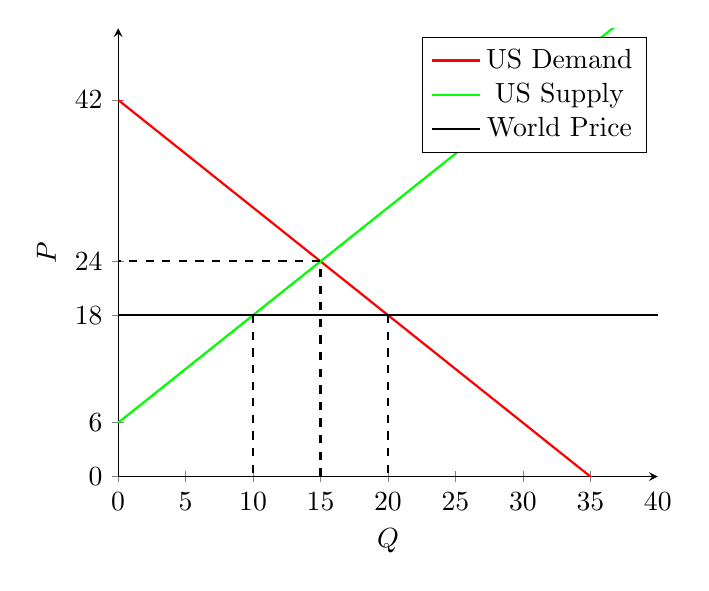
\begin{tikzpicture}
        \begin{axis}[
            axis lines = left,
            xlabel = $Q$,
            ylabel = $P$,
            ymax = 50,
            ymin = 0,
            xmax = 40,
            xmin = 0,
            scaled x ticks = false,
            ytick = {0,6,18,24,42},
            xtick = {0,5,10,15,20,25,30,35,40}
        ]
        \addplot[
        color=red,thick,
        domain=0:50,
        range = 0:50]{-18*x/15 + 42};
        \addlegendentry{US Demand}
        \addplot[
        color=green,thick,
        domain=0:50,
        range = 0:50]{18*x/15 + 6};
        \addlegendentry{US Supply}
        \addplot[
        color=black,thick,
        domain=0:50,
        range = 0:50]{18};
        \addlegendentry{World Price}
        \addplot[
        black,thick,dashed]
        coordinates {
            (15,0)
            (15,24)
            (0,24)
        };
        \addplot[
        black,thick,dashed]
        coordinates {
            (10,18)
            (10,0)
        };
        \addplot[
        black,thick,dashed]
        coordinates {
            (20,18)
            (20,0)
        };
        \end{axis}
        \end{tikzpicture}
    \end{center}
\end{frame}

\begin{frame}{Wing\$}
    Under autarky, the consumer surplus is?
    \begin{center}
        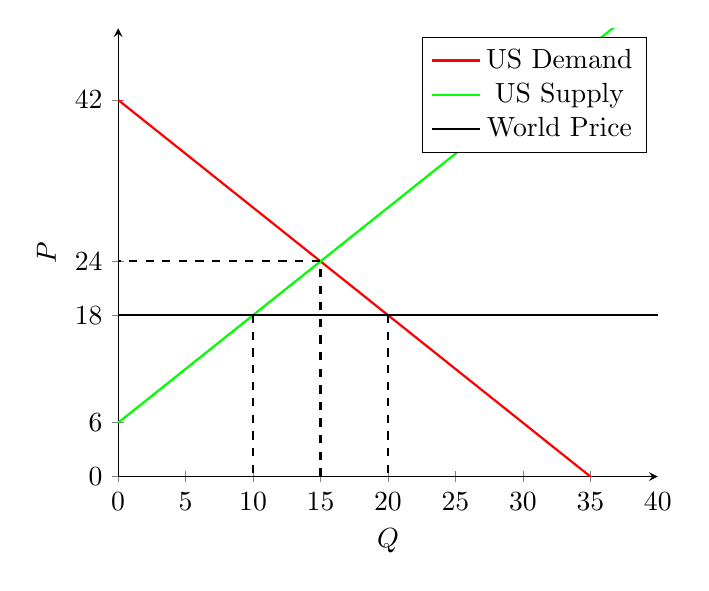
\begin{tikzpicture}
        \begin{axis}[
            axis lines = left,
            xlabel = $Q$,
            ylabel = $P$,
            ymax = 50,
            ymin = 0,
            xmax = 40,
            xmin = 0,
            scaled x ticks = false,
            ytick = {0,6,18,24,42},
            xtick = {0,5,10,15,20,25,30,35,40}
        ]
        \addplot[
        color=red,thick,
        domain=0:50,
        range = 0:50]{-18*x/15 + 42};
        \addlegendentry{US Demand}
        \addplot[
        color=green,thick,
        domain=0:50,
        range = 0:50]{18*x/15 + 6};
        \addlegendentry{US Supply}
        \addplot[
        color=black,thick,
        domain=0:50,
        range = 0:50]{18};
        \addlegendentry{World Price}
        \addplot[
        black,thick,dashed]
        coordinates {
            (15,0)
            (15,24)
            (0,24)
        };
        \addplot[
        black,thick,dashed]
        coordinates {
            (10,18)
            (10,0)
        };
        \addplot[
        black,thick,dashed]
        coordinates {
            (20,18)
            (20,0)
        };
        \end{axis}
        \end{tikzpicture}
    \end{center}
\end{frame}

\begin{frame}[t]{Wing\$}
    \textbf{Under autarky, the consumer surplus is?}
    \newline
    \newline
    We use our traditional triangle formulation at the equilibrium of the US market (as there is no trade:
    \[\begin{split}
        CS &= \frac{(\$42-\$24)(15)}{2} \\
        &= \frac{(\$18)(15)}{2} \\
        &= \boxed{\$135} \\
    \end{split}\]
\end{frame}

\begin{frame}{Wing\$}
    Under autarky, the producer surplus is?
    \begin{center}
        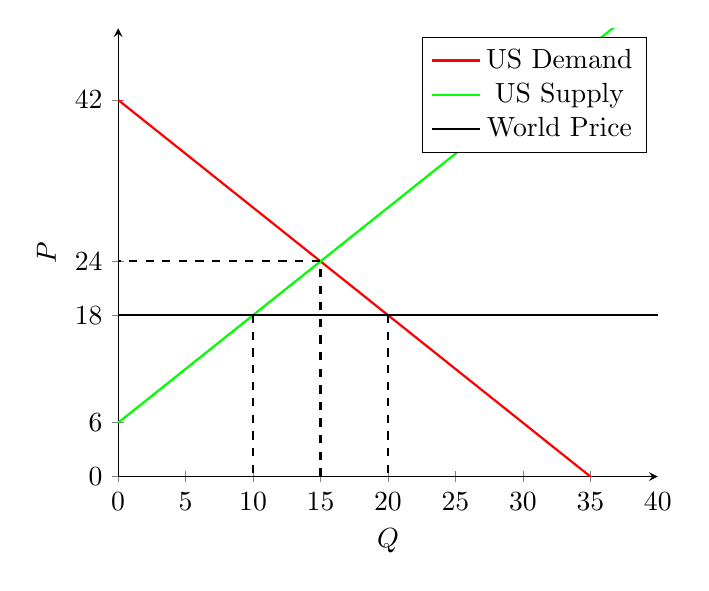
\begin{tikzpicture}
        \begin{axis}[
            axis lines = left,
            xlabel = $Q$,
            ylabel = $P$,
            ymax = 50,
            ymin = 0,
            xmax = 40,
            xmin = 0,
            scaled x ticks = false,
            ytick = {0,6,18,24,42},
            xtick = {0,5,10,15,20,25,30,35,40}
        ]
        \addplot[
        color=red,thick,
        domain=0:50,
        range = 0:50]{-18*x/15 + 42};
        \addlegendentry{US Demand}
        \addplot[
        color=green,thick,
        domain=0:50,
        range = 0:50]{18*x/15 + 6};
        \addlegendentry{US Supply}
        \addplot[
        color=black,thick,
        domain=0:50,
        range = 0:50]{18};
        \addlegendentry{World Price}
        \addplot[
        black,thick,dashed]
        coordinates {
            (15,0)
            (15,24)
            (0,24)
        };
        \addplot[
        black,thick,dashed]
        coordinates {
            (10,18)
            (10,0)
        };
        \addplot[
        black,thick,dashed]
        coordinates {
            (20,18)
            (20,0)
        };
        \end{axis}
        \end{tikzpicture}
    \end{center}
\end{frame}

\begin{frame}[t]{Wing\$}
    \textbf{Under autarky, the producer surplus is?}
    \newline
    \newline As there is no trade, this is just the producer surplus in the US market:
    \[\begin{split}
        PS &= \frac{(\$24 - \$6) 15}{2} \\
        &= \frac{(\$18)(15)}{2} \\
        &= \boxed{\$135}
    \end{split}\]
\end{frame}

\begin{frame}{Wing\$}
    Under autarky, the deadweight loss is?
    \begin{center}
        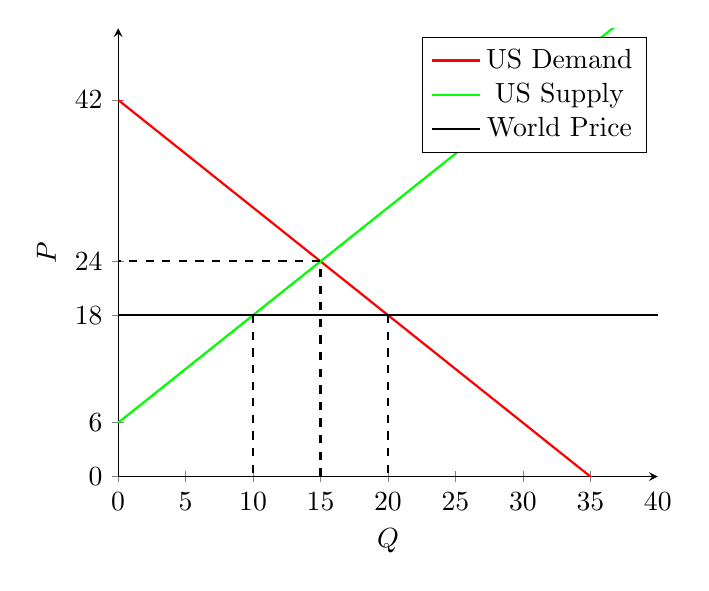
\begin{tikzpicture}
        \begin{axis}[
            axis lines = left,
            xlabel = $Q$,
            ylabel = $P$,
            ymax = 50,
            ymin = 0,
            xmax = 40,
            xmin = 0,
            scaled x ticks = false,
            ytick = {0,6,18,24,42},
            xtick = {0,5,10,15,20,25,30,35,40}
        ]
        \addplot[
        color=red,thick,
        domain=0:50,
        range = 0:50]{-18*x/15 + 42};
        \addlegendentry{US Demand}
        \addplot[
        color=green,thick,
        domain=0:50,
        range = 0:50]{18*x/15 + 6};
        \addlegendentry{US Supply}
        \addplot[
        color=black,thick,
        domain=0:50,
        range = 0:50]{18};
        \addlegendentry{World Price}
        \addplot[
        black,thick,dashed]
        coordinates {
            (15,0)
            (15,24)
            (0,24)
        };
        \addplot[
        black,thick,dashed]
        coordinates {
            (10,18)
            (10,0)
        };
        \addplot[
        black,thick,dashed]
        coordinates {
            (20,18)
            (20,0)
        };
        \end{axis}
        \end{tikzpicture}
    \end{center}
\end{frame}

\begin{frame}{Wing\$}
    If the US Government allows imports, what will the market price, $Q_D$, and $Q_S$ be?
    \begin{center}
        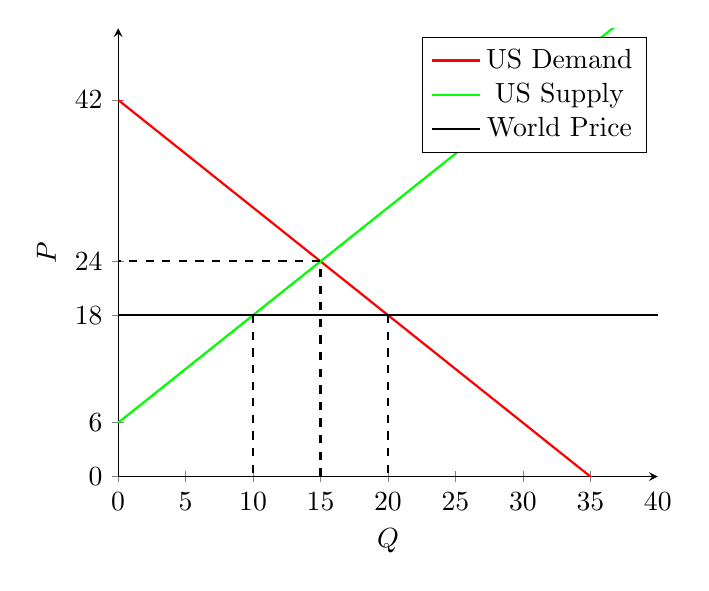
\begin{tikzpicture}
        \begin{axis}[
            axis lines = left,
            xlabel = $Q$,
            ylabel = $P$,
            ymax = 50,
            ymin = 0,
            xmax = 40,
            xmin = 0,
            scaled x ticks = false,
            ytick = {0,6,18,24,42},
            xtick = {0,5,10,15,20,25,30,35,40}
        ]
        \addplot[
        color=red,thick,
        domain=0:50,
        range = 0:50]{-18*x/15 + 42};
        \addlegendentry{US Demand}
        \addplot[
        color=green,thick,
        domain=0:50,
        range = 0:50]{18*x/15 + 6};
        \addlegendentry{US Supply}
        \addplot[
        color=black,thick,
        domain=0:50,
        range = 0:50]{18};
        \addlegendentry{World Price}
        \addplot[
        black,thick,dashed]
        coordinates {
            (15,0)
            (15,24)
            (0,24)
        };
        \addplot[
        black,thick,dashed]
        coordinates {
            (10,18)
            (10,0)
        };
        \addplot[
        black,thick,dashed]
        coordinates {
            (20,18)
            (20,0)
        };
        \end{axis}
        \end{tikzpicture}
    \end{center}
\end{frame}

\begin{frame}{Wing\$}
    If the US Government allows imports, how much will be supplied domestically vs. imported? What is domestic producer surplus?
    \begin{center}
        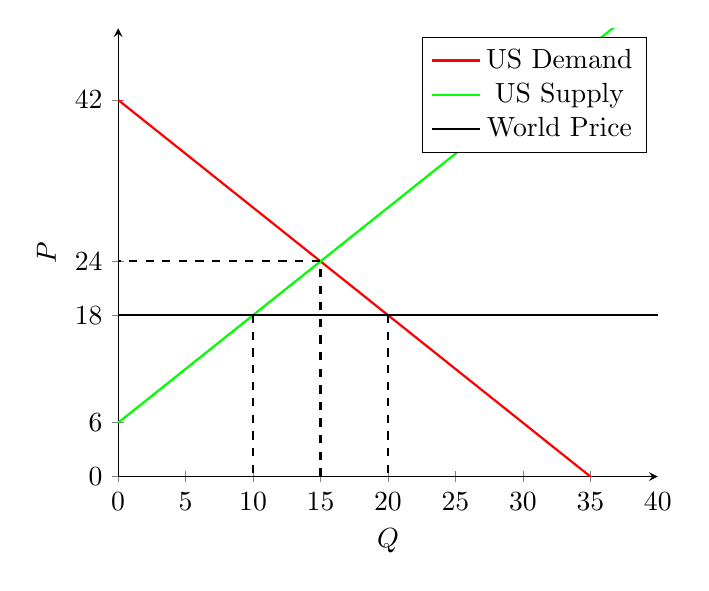
\begin{tikzpicture}
        \begin{axis}[
            axis lines = left,
            xlabel = $Q$,
            ylabel = $P$,
            ymax = 50,
            ymin = 0,
            xmax = 40,
            xmin = 0,
            scaled x ticks = false,
            ytick = {0,6,18,24,42},
            xtick = {0,5,10,15,20,25,30,35,40}
        ]
        \addplot[
        color=red,thick,
        domain=0:50,
        range = 0:50]{-18*x/15 + 42};
        \addlegendentry{US Demand}
        \addplot[
        color=green,thick,
        domain=0:50,
        range = 0:50]{18*x/15 + 6};
        \addlegendentry{US Supply}
        \addplot[
        color=black,thick,
        domain=0:50,
        range = 0:50]{18};
        \addlegendentry{World Price}
        \addplot[
        black,thick,dashed]
        coordinates {
            (15,0)
            (15,24)
            (0,24)
        };
        \addplot[
        black,thick,dashed]
        coordinates {
            (10,18)
            (10,0)
        };
        \addplot[
        black,thick,dashed]
        coordinates {
            (20,18)
            (20,0)
        };
        \end{axis}
        \end{tikzpicture}
    \end{center}
\end{frame}

\begin{frame}[t]{Wing\$}
    \textbf{Domestic Producer Surplus}
    \newline
    \newline As the domestic producers are now only producing 10 at the market price of \$18, we can assess the smaller surplus with our triangle area formula:
    \[\begin{split}
        PS_{domestic} &= \frac{(\$18-\$6)(10)}{2} \\
        &= \frac{(\$12)(10)}{2} \\
        &= \boxed{\$60}
    \end{split}\]
\end{frame}

\begin{frame}{Wing\$}
    If the US Government allows imports, what is the consumer surplus?
    \begin{center}
        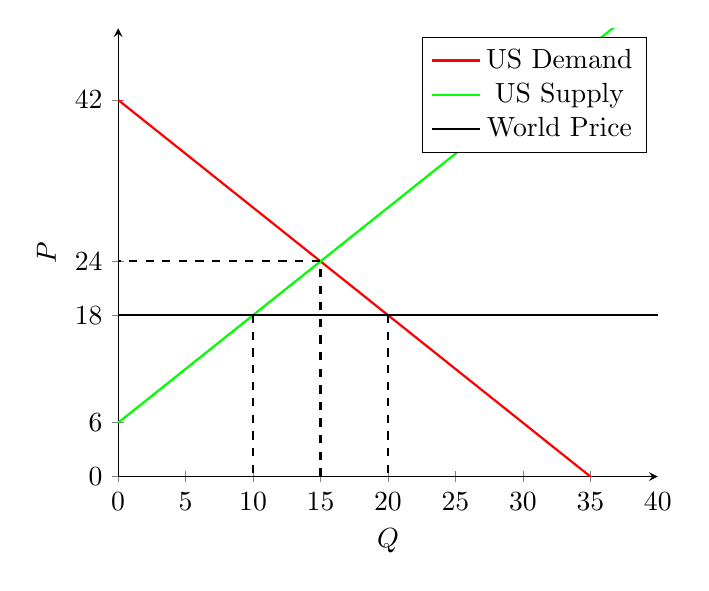
\begin{tikzpicture}
        \begin{axis}[
            axis lines = left,
            xlabel = $Q$,
            ylabel = $P$,
            ymax = 50,
            ymin = 0,
            xmax = 40,
            xmin = 0,
            scaled x ticks = false,
            ytick = {0,6,18,24,42},
            xtick = {0,5,10,15,20,25,30,35,40}
        ]
        \addplot[
        color=red,thick,
        domain=0:50,
        range = 0:50]{-18*x/15 + 42};
        \addlegendentry{US Demand}
        \addplot[
        color=green,thick,
        domain=0:50,
        range = 0:50]{18*x/15 + 6};
        \addlegendentry{US Supply}
        \addplot[
        color=black,thick,
        domain=0:50,
        range = 0:50]{18};
        \addlegendentry{World Price}
        \addplot[
        black,thick,dashed]
        coordinates {
            (15,0)
            (15,24)
            (0,24)
        };
        \addplot[
        black,thick,dashed]
        coordinates {
            (10,18)
            (10,0)
        };
        \addplot[
        black,thick,dashed]
        coordinates {
            (20,18)
            (20,0)
        };
        \end{axis}
        \end{tikzpicture}
    \end{center}
\end{frame}

\begin{frame}[t]{Wing\$}
    \textbf{What is the consumer surplus if imports are allowed?}
    \newline
    \newline Now the consumers consume 20 units at a price of \$18, so we have
    \[\begin{split}
        CS &= \frac{(\$42- \$18) 20}{2} \\
        &= \frac{(\$24) (20)}{2} \\
        &= \boxed{\$240}
    \end{split}\]
\end{frame}

\begin{frame}{Sugar, We're Goin Down}
    US Market for sugar
    \begin{center}
        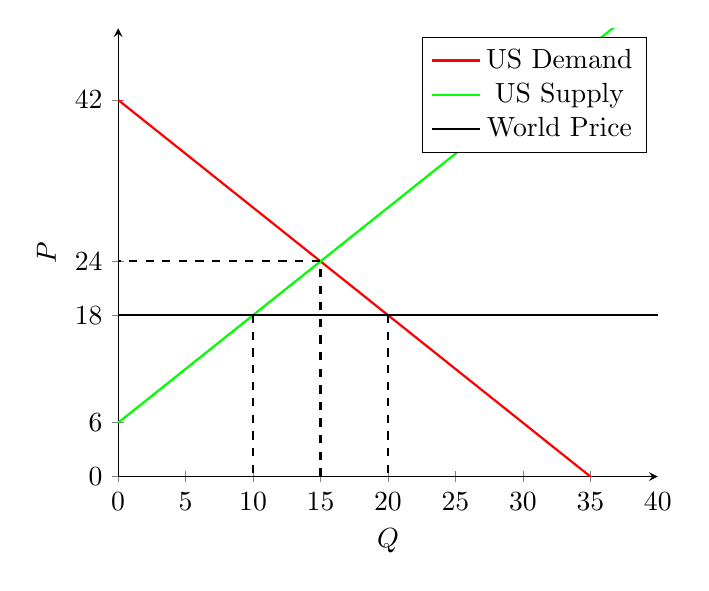
\begin{tikzpicture}
        \begin{axis}[
            axis lines = left,
            xlabel = $Q$,
            ylabel = $P$,
            ymax = 50,
            ymin = 0,
            xmax = 40,
            xmin = 0,
            scaled x ticks = false,
            ytick = {0,6,18,24,42},
            xtick = {0,5,10,15,20,25,30,35,40}
        ]
        \addplot[
        color=red,thick,
        domain=0:50,
        range = 0:50]{-18*x/15 + 42};
        \addlegendentry{US Demand}
        \addplot[
        color=green,thick,
        domain=0:50,
        range = 0:50]{18*x/15 + 6};
        \addlegendentry{US Supply}
        \addplot[
        color=black,thick,
        domain=0:50,
        range = 0:50]{18};
        \addlegendentry{World Price}
        \addplot[
        black,thick,dashed]
        coordinates {
            (15,0)
            (15,24)
            (0,24)
        };
        \addplot[
        black,thick,dashed]
        coordinates {
            (10,18)
            (10,0)
        };
        \addplot[
        black,thick,dashed]
        coordinates {
            (20,18)
            (20,0)
        };
        \end{axis}
        \end{tikzpicture}
    \end{center}
\end{frame}

\begin{frame}{Sugar, We're Goin Down}
    Following the imposition of the tariff, what is the price that domestic consumers must now pay and what is the quantity purchased?
        \begin{center}
        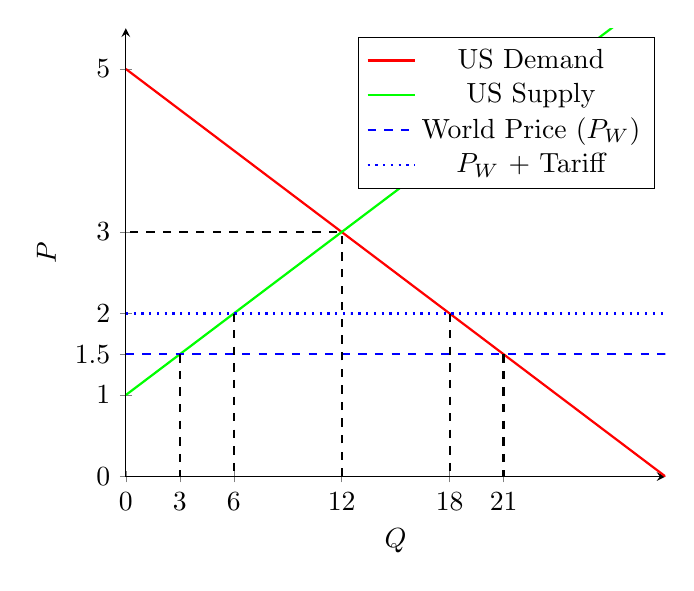
\begin{tikzpicture}
        \begin{axis}[
            axis lines = left,
            xlabel = $Q$,
            ylabel = $P$,
            ymax = 5.5,
            ymin = 0,
            xmax = 30,
            xmin = 0,
            scaled x ticks = false,
            ytick = {0,1,1.5,2,3,5},
            xtick = {0,3,6,12,18,21}
        ]
        \addplot[
        color=red,thick,
        domain=0:50,
        range = 0:50]{-x/6 + 5};
        \addlegendentry{US Demand}
        \addplot[
        color=green,thick,
        domain=0:50,
        range = 0:50]{x/6 + 1};
        \addlegendentry{US Supply}
        \addplot[
        color=blue,thick,dashed,
        domain=0:50,
        range = 0:50]{1.5};
        \addlegendentry{{World Price ($P_W$)}}
        \addplot[
        color=blue,thick,dotted,
        domain=0:50,
        range = 0:50]{2};
        \addlegendentry{{$P_W$ + Tariff}}
        \addplot[
        black,thick,dashed]
        coordinates {
            (12,0)
            (12,3)
            (0,3)
        };
        \addplot[
        black,thick,dashed]
        coordinates {
            (3,1.5)
            (3,0)
        };
        \addplot[
        black,thick,dashed]
        coordinates {
            (21,1.5)
            (21,0)
        };
        \addplot[
        black,thick,dashed]
        coordinates {
            (6,2)
            (6,0)
        };
        \addplot[
        black,thick,dashed]
        coordinates {
            (18,2)
            (18,0)
        };
        \end{axis}
        \end{tikzpicture}
    \end{center}
\end{frame}

\begin{frame}{Sugar, We're Goin Down}
    Calculate the value of consumer surplus with the tariff in place.
        \begin{center}
        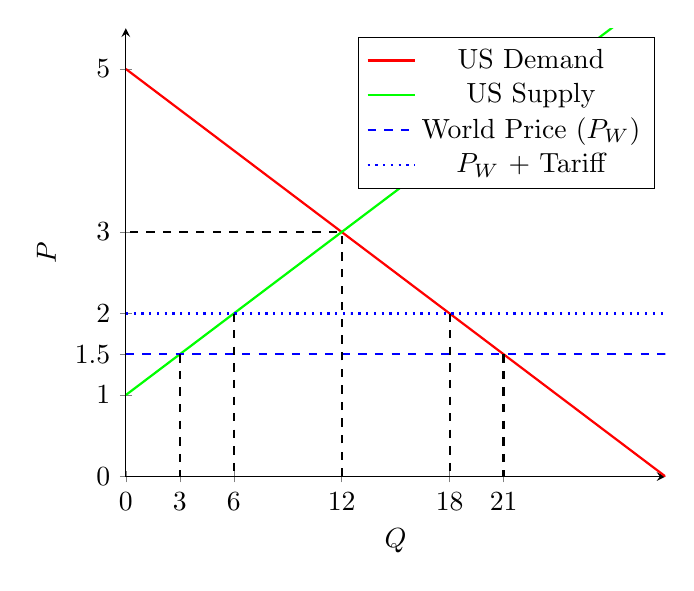
\begin{tikzpicture}
        \begin{axis}[
            axis lines = left,
            xlabel = $Q$,
            ylabel = $P$,
            ymax = 5.5,
            ymin = 0,
            xmax = 30,
            xmin = 0,
            scaled x ticks = false,
            ytick = {0,1,1.5,2,3,5},
            xtick = {0,3,6,12,18,21}
        ]
        \addplot[
        color=red,thick,
        domain=0:50,
        range = 0:50]{-x/6 + 5};
        \addlegendentry{US Demand}
        \addplot[
        color=green,thick,
        domain=0:50,
        range = 0:50]{x/6 + 1};
        \addlegendentry{US Supply}
        \addplot[
        color=blue,thick,dashed,
        domain=0:50,
        range = 0:50]{1.5};
        \addlegendentry{{World Price ($P_W$)}}
        \addplot[
        color=blue,thick,dotted,
        domain=0:50,
        range = 0:50]{2};
        \addlegendentry{{$P_W$ + Tariff}}
        \addplot[
        black,thick,dashed]
        coordinates {
            (12,0)
            (12,3)
            (0,3)
        };
        \addplot[
        black,thick,dashed]
        coordinates {
            (3,1.5)
            (3,0)
        };
        \addplot[
        black,thick,dashed]
        coordinates {
            (21,1.5)
            (21,0)
        };
        \addplot[
        black,thick,dashed]
        coordinates {
            (6,2)
            (6,0)
        };
        \addplot[
        black,thick,dashed]
        coordinates {
            (18,2)
            (18,0)
        };
        \end{axis}
        \end{tikzpicture}
    \end{center}
\end{frame}

\begin{frame}[t]{Sugar, We're Goin Down}
    \textbf{Calculate the value of consumer surplus with the tariff in place.}
    \newline
    \newline We use our traditional area formula at the price and quantity calculated previously:
    \[\begin{split}
        CS_{tariff} &= \frac{(\$5-\$2)(18)}{2} \\
        &= \frac{(\$3)(18)}{2} \\
        &= \boxed{\$27}
    \end{split}\]
\end{frame}

\begin{frame}{Sugar, We're Goin Down}
    What is the quantity supplied by domestic sugar producers with the tariff in place?
        \begin{center}
        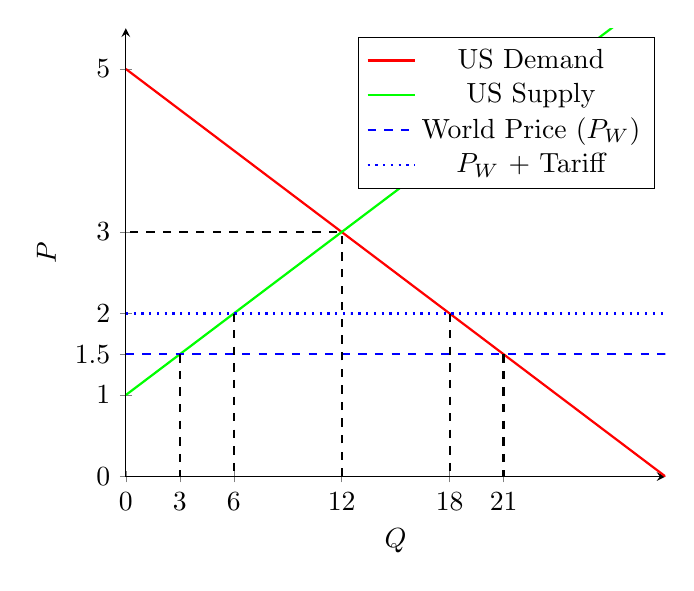
\begin{tikzpicture}
        \begin{axis}[
            axis lines = left,
            xlabel = $Q$,
            ylabel = $P$,
            ymax = 5.5,
            ymin = 0,
            xmax = 30,
            xmin = 0,
            scaled x ticks = false,
            ytick = {0,1,1.5,2,3,5},
            xtick = {0,3,6,12,18,21}
        ]
        \addplot[
        color=red,thick,
        domain=0:50,
        range = 0:50]{-x/6 + 5};
        \addlegendentry{US Demand}
        \addplot[
        color=green,thick,
        domain=0:50,
        range = 0:50]{x/6 + 1};
        \addlegendentry{US Supply}
        \addplot[
        color=blue,thick,dashed,
        domain=0:50,
        range = 0:50]{1.5};
        \addlegendentry{{World Price ($P_W$)}}
        \addplot[
        color=blue,thick,dotted,
        domain=0:50,
        range = 0:50]{2};
        \addlegendentry{{$P_W$ + Tariff}}
        \addplot[
        black,thick,dashed]
        coordinates {
            (12,0)
            (12,3)
            (0,3)
        };
        \addplot[
        black,thick,dashed]
        coordinates {
            (3,1.5)
            (3,0)
        };
        \addplot[
        black,thick,dashed]
        coordinates {
            (21,1.5)
            (21,0)
        };
        \addplot[
        black,thick,dashed]
        coordinates {
            (6,2)
            (6,0)
        };
        \addplot[
        black,thick,dashed]
        coordinates {
            (18,2)
            (18,0)
        };
        \end{axis}
        \end{tikzpicture}
    \end{center}
\end{frame}

\begin{frame}{Sugar, We're Goin Down}
   Calculate the value of producer surplus received by U.S. sugar producers with the tariff in place.
        \begin{center}
        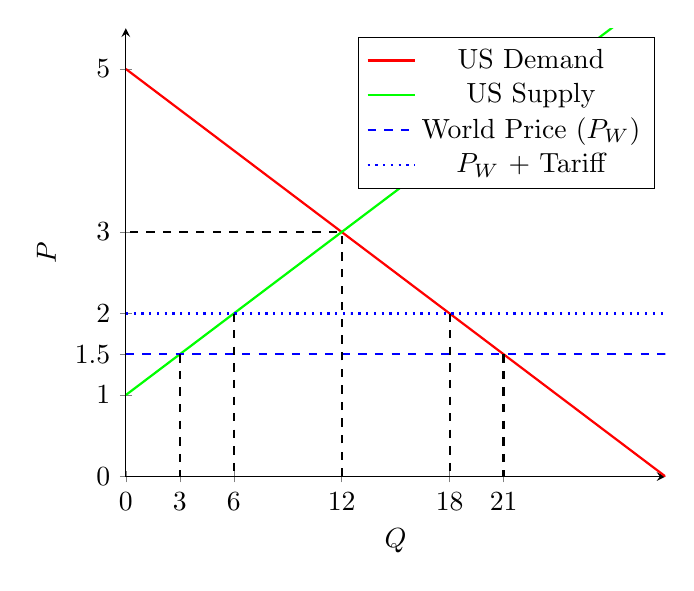
\begin{tikzpicture}
        \begin{axis}[
            axis lines = left,
            xlabel = $Q$,
            ylabel = $P$,
            ymax = 5.5,
            ymin = 0,
            xmax = 30,
            xmin = 0,
            scaled x ticks = false,
            ytick = {0,1,1.5,2,3,5},
            xtick = {0,3,6,12,18,21}
        ]
        \addplot[
        color=red,thick,
        domain=0:50,
        range = 0:50]{-x/6 + 5};
        \addlegendentry{US Demand}
        \addplot[
        color=green,thick,
        domain=0:50,
        range = 0:50]{x/6 + 1};
        \addlegendentry{US Supply}
        \addplot[
        color=blue,thick,dashed,
        domain=0:50,
        range = 0:50]{1.5};
        \addlegendentry{{World Price ($P_W$)}}
        \addplot[
        color=blue,thick,dotted,
        domain=0:50,
        range = 0:50]{2};
        \addlegendentry{{$P_W$ + Tariff}}
        \addplot[
        black,thick,dashed]
        coordinates {
            (12,0)
            (12,3)
            (0,3)
        };
        \addplot[
        black,thick,dashed]
        coordinates {
            (3,1.5)
            (3,0)
        };
        \addplot[
        black,thick,dashed]
        coordinates {
            (21,1.5)
            (21,0)
        };
        \addplot[
        black,thick,dashed]
        coordinates {
            (6,2)
            (6,0)
        };
        \addplot[
        black,thick,dashed]
        coordinates {
            (18,2)
            (18,0)
        };
        \end{axis}
        \end{tikzpicture}
    \end{center}
\end{frame}

\begin{frame}[t]{Sugar, We're Goin Down}
    \textbf{Calculate the value of producer surplus received by U.S. sugar producers with the tariff in place.} 
    \newline
    \newline Under the tariff, U.S. producers supply 6 units at a price of \$2, so we have
    \[\begin{split}
        PS_{tariff} &= \frac{(\$2 - \$1)6}{2}\\
        &= \frac{(\$1)6}{2}\\
        &= \boxed{\$3}
    \end{split}\]
\end{frame}

\begin{frame}{Sugar, We're Goin Down}
   What is the quantity of sugar imported with the tariff in place?
        \begin{center}
        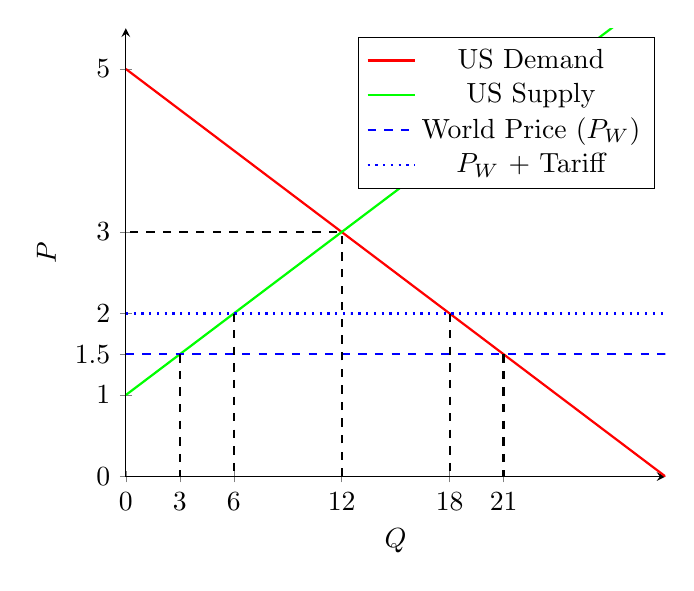
\begin{tikzpicture}
        \begin{axis}[
            axis lines = left,
            xlabel = $Q$,
            ylabel = $P$,
            ymax = 5.5,
            ymin = 0,
            xmax = 30,
            xmin = 0,
            scaled x ticks = false,
            ytick = {0,1,1.5,2,3,5},
            xtick = {0,3,6,12,18,21}
        ]
        \addplot[
        color=red,thick,
        domain=0:50,
        range = 0:50]{-x/6 + 5};
        \addlegendentry{US Demand}
        \addplot[
        color=green,thick,
        domain=0:50,
        range = 0:50]{x/6 + 1};
        \addlegendentry{US Supply}
        \addplot[
        color=blue,thick,dashed,
        domain=0:50,
        range = 0:50]{1.5};
        \addlegendentry{{World Price ($P_W$)}}
        \addplot[
        color=blue,thick,dotted,
        domain=0:50,
        range = 0:50]{2};
        \addlegendentry{{$P_W$ + Tariff}}
        \addplot[
        black,thick,dashed]
        coordinates {
            (12,0)
            (12,3)
            (0,3)
        };
        \addplot[
        black,thick,dashed]
        coordinates {
            (3,1.5)
            (3,0)
        };
        \addplot[
        black,thick,dashed]
        coordinates {
            (21,1.5)
            (21,0)
        };
        \addplot[
        black,thick,dashed]
        coordinates {
            (6,2)
            (6,0)
        };
        \addplot[
        black,thick,dashed]
        coordinates {
            (18,2)
            (18,0)
        };
        \end{axis}
        \end{tikzpicture}
    \end{center}
\end{frame}

\begin{frame}{Sugar, We're Goin Down}
   What is the amount of tariff revenue collected by the government?
        \begin{center}
        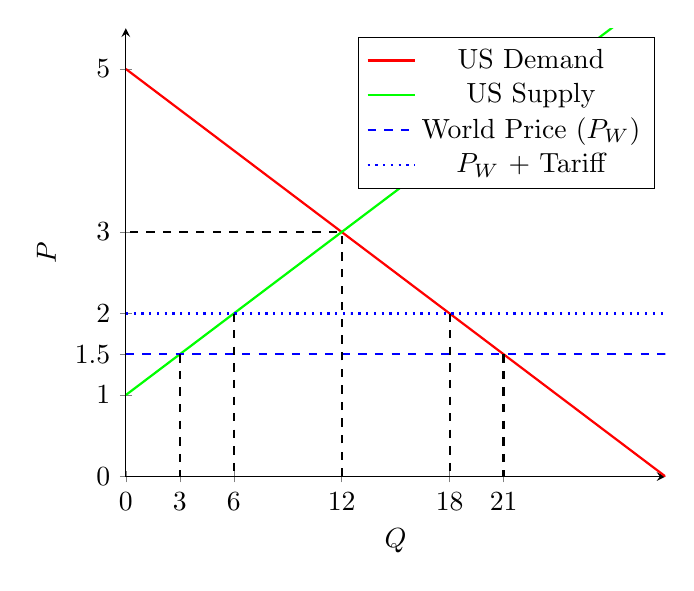
\begin{tikzpicture}
        \begin{axis}[
            axis lines = left,
            xlabel = $Q$,
            ylabel = $P$,
            ymax = 5.5,
            ymin = 0,
            xmax = 30,
            xmin = 0,
            scaled x ticks = false,
            ytick = {0,1,1.5,2,3,5},
            xtick = {0,3,6,12,18,21}
        ]
        \addplot[
        color=red,thick,
        domain=0:50,
        range = 0:50]{-x/6 + 5};
        \addlegendentry{US Demand}
        \addplot[
        color=green,thick,
        domain=0:50,
        range = 0:50]{x/6 + 1};
        \addlegendentry{US Supply}
        \addplot[
        color=blue,thick,dashed,
        domain=0:50,
        range = 0:50]{1.5};
        \addlegendentry{{World Price ($P_W$)}}
        \addplot[
        color=blue,thick,dotted,
        domain=0:50,
        range = 0:50]{2};
        \addlegendentry{{$P_W$ + Tariff}}
        \addplot[
        black,thick,dashed]
        coordinates {
            (12,0)
            (12,3)
            (0,3)
        };
        \addplot[
        black,thick,dashed]
        coordinates {
            (3,1.5)
            (3,0)
        };
        \addplot[
        black,thick,dashed]
        coordinates {
            (21,1.5)
            (21,0)
        };
        \addplot[
        black,thick,dashed]
        coordinates {
            (6,2)
            (6,0)
        };
        \addplot[
        black,thick,dashed]
        coordinates {
            (18,2)
            (18,0)
        };
        \end{axis}
        \end{tikzpicture}
    \end{center}
\end{frame}

\begin{frame}[t]{Sugar, We're Goin Down}
    \textbf{What is the amount of tariff revenue collected by the government?}
    \newline
    \newline This is just the size of the tariff multiplied by the amount imported:
    \[\begin{split}
        \text{Tariff Revenue} &= (18-6) \times \$.5 \\
        &= \boxed{\$6}
    \end{split}\]
\end{frame}

\begin{frame}{Sugar, We're Goin Down}
    The tariff has reduced consumer surplus. Calculate the loss in consumer surplus due to the tariff.
        \begin{center}
        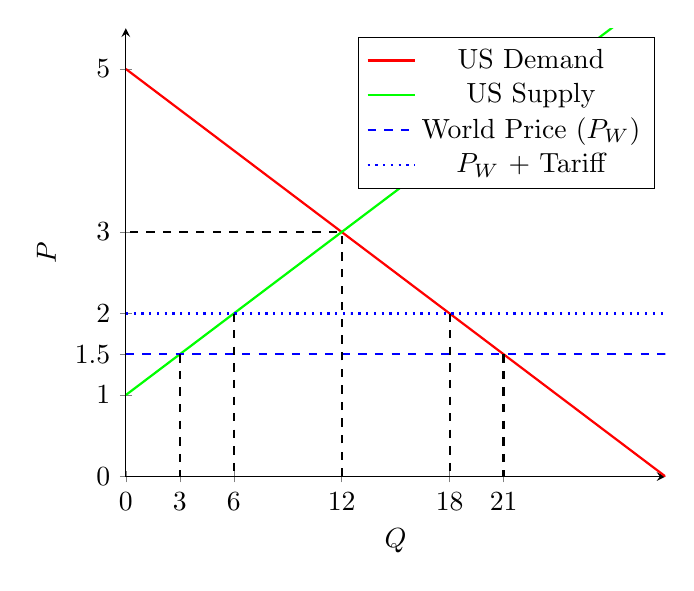
\begin{tikzpicture}
        \begin{axis}[
            axis lines = left,
            xlabel = $Q$,
            ylabel = $P$,
            ymax = 5.5,
            ymin = 0,
            xmax = 30,
            xmin = 0,
            scaled x ticks = false,
            ytick = {0,1,1.5,2,3,5},
            xtick = {0,3,6,12,18,21}
        ]
        \addplot[
        color=red,thick,
        domain=0:50,
        range = 0:50]{-x/6 + 5};
        \addlegendentry{US Demand}
        \addplot[
        color=green,thick,
        domain=0:50,
        range = 0:50]{x/6 + 1};
        \addlegendentry{US Supply}
        \addplot[
        color=blue,thick,dashed,
        domain=0:50,
        range = 0:50]{1.5};
        \addlegendentry{{World Price ($P_W$)}}
        \addplot[
        color=blue,thick,dotted,
        domain=0:50,
        range = 0:50]{2};
        \addlegendentry{{$P_W$ + Tariff}}
        \addplot[
        black,thick,dashed]
        coordinates {
            (12,0)
            (12,3)
            (0,3)
        };
        \addplot[
        black,thick,dashed]
        coordinates {
            (3,1.5)
            (3,0)
        };
        \addplot[
        black,thick,dashed]
        coordinates {
            (21,1.5)
            (21,0)
        };
        \addplot[
        black,thick,dashed]
        coordinates {
            (6,2)
            (6,0)
        };
        \addplot[
        black,thick,dashed]
        coordinates {
            (18,2)
            (18,0)
        };
        \end{axis}
        \end{tikzpicture}
    \end{center}
\end{frame}

\begin{frame}[t]{Sugar, We're Goin Down}
    \textbf{The tariff has reduced consumer surplus. Calculate the loss in consumer surplus due to the tariff.}
    \newline
    \newline We compute the difference between consumer surplus before and after the tariff:
    \[\begin{split}
        CS_{diff} &= CS_{pre} - CS_{post} \\
        &= \frac{(\$5 - \$1.5)21}{2} - \frac{(\$5 - \$2)18}{2} \\
        &= \frac{(\$3.5)21}{2} - \frac{(\$3)18}{2} \\
        &= \$36.75 - \$27 \\
        &= \boxed{\$9.25}
    \end{split}\]
\end{frame}

\begin{frame}{Sugar, We're Goin Down}
    What portion of the consumer surplus loss is redistributed to domestic producers? To the government?
        \begin{center}
        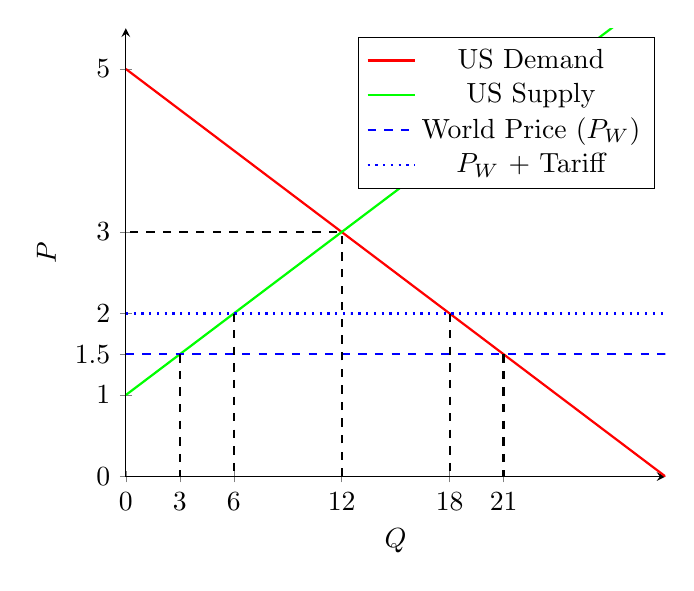
\begin{tikzpicture}
        \begin{axis}[
            axis lines = left,
            xlabel = $Q$,
            ylabel = $P$,
            ymax = 5.5,
            ymin = 0,
            xmax = 30,
            xmin = 0,
            scaled x ticks = false,
            ytick = {0,1,1.5,2,3,5},
            xtick = {0,3,6,12,18,21}
        ]
        \addplot[
        color=red,thick,
        domain=0:50,
        range = 0:50]{-x/6 + 5};
        \addlegendentry{US Demand}
        \addplot[
        color=green,thick,
        domain=0:50,
        range = 0:50]{x/6 + 1};
        \addlegendentry{US Supply}
        \addplot[
        color=blue,thick,dashed,
        domain=0:50,
        range = 0:50]{1.5};
        \addlegendentry{{World Price ($P_W$)}}
        \addplot[
        color=blue,thick,dotted,
        domain=0:50,
        range = 0:50]{2};
        \addlegendentry{{$P_W$ + Tariff}}
        \addplot[
        black,thick,dashed]
        coordinates {
            (12,0)
            (12,3)
            (0,3)
        };
        \addplot[
        black,thick,dashed]
        coordinates {
            (3,1.5)
            (3,0)
        };
        \addplot[
        black,thick,dashed]
        coordinates {
            (21,1.5)
            (21,0)
        };
        \addplot[
        black,thick,dashed]
        coordinates {
            (6,2)
            (6,0)
        };
        \addplot[
        black,thick,dashed]
        coordinates {
            (18,2)
            (18,0)
        };
        \end{axis}
        \end{tikzpicture}
    \end{center}
\end{frame}

\begin{frame}[t]{Sugar, We're Goin Down}
    \textbf{What portion of the consumer surplus loss is redistributed to domestic producers? To the government?}
    \newline
    \newline The government is easier to start with, as it's just the tariff that the government receives. We calculated this earlier to be \$6. The portion that the producers receive is the difference between their surplus before and after the tariff:
    \[\begin{split}
        CS_{diff} &= CS_{post} - CS_{pre} \\
        &= \frac{(\$2-\$1)6}{2} - \frac{(\$1.5 - \$1)3}{2} \\
        &= \$3- \$.75 \\
        &= \boxed{\$2.25}
    \end{split}\]
\end{frame}

\begin{frame}{Sugar, We're Goin Down}
    Calculate the deadweight loss due to the tariff.
        \begin{center}
        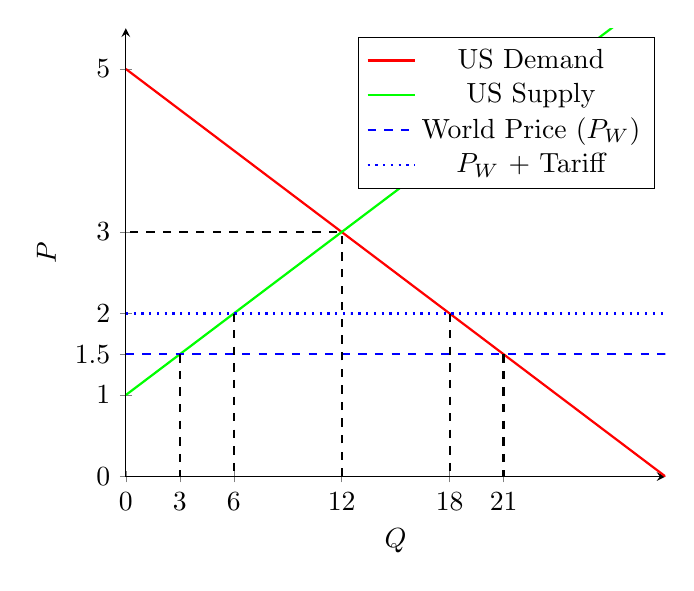
\begin{tikzpicture}
        \begin{axis}[
            axis lines = left,
            xlabel = $Q$,
            ylabel = $P$,
            ymax = 5.5,
            ymin = 0,
            xmax = 30,
            xmin = 0,
            scaled x ticks = false,
            ytick = {0,1,1.5,2,3,5},
            xtick = {0,3,6,12,18,21}
        ]
        \addplot[
        color=red,thick,
        domain=0:50,
        range = 0:50]{-x/6 + 5};
        \addlegendentry{US Demand}
        \addplot[
        color=green,thick,
        domain=0:50,
        range = 0:50]{x/6 + 1};
        \addlegendentry{US Supply}
        \addplot[
        color=blue,thick,dashed,
        domain=0:50,
        range = 0:50]{1.5};
        \addlegendentry{{World Price ($P_W$)}}
        \addplot[
        color=blue,thick,dotted,
        domain=0:50,
        range = 0:50]{2};
        \addlegendentry{{$P_W$ + Tariff}}
        \addplot[
        black,thick,dashed]
        coordinates {
            (12,0)
            (12,3)
            (0,3)
        };
        \addplot[
        black,thick,dashed]
        coordinates {
            (3,1.5)
            (3,0)
        };
        \addplot[
        black,thick,dashed]
        coordinates {
            (21,1.5)
            (21,0)
        };
        \addplot[
        black,thick,dashed]
        coordinates {
            (6,2)
            (6,0)
        };
        \addplot[
        black,thick,dashed]
        coordinates {
            (18,2)
            (18,0)
        };
        \end{axis}
        \end{tikzpicture}
    \end{center}
\end{frame}

\begin{frame}{Bragabong}
    Bragabong currently both produces and imports almonds. The government decides to restrict international trade in almonds by imposing a quota allowing imports of only 10 million kilos each year.
    \begin{center}
        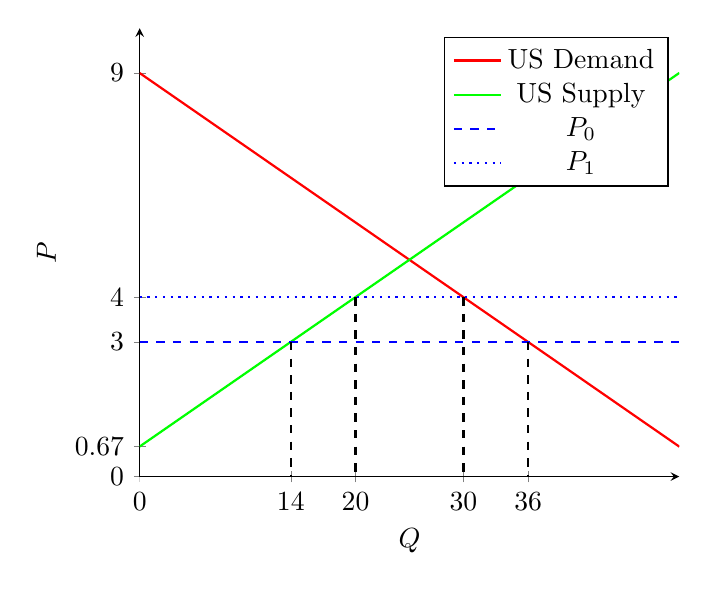
\begin{tikzpicture}
        \begin{axis}[
            axis lines = left,
            xlabel = $Q$,
            ylabel = $P$,
            ymax = 10,
            ymin = 0,
            xmax = 50,
            xmin = 0,
            scaled x ticks = false,
            ytick = {0,.67, 3,4,9},
            xtick = {0,14,20,30,36}
        ]
        \addplot[
        color=red,thick,
        domain=0:50,
        range = 0:50]{-x/6 + 9};
        \addlegendentry{US Demand}
        \addplot[
        color=green,thick,
        domain=0:50,
        range = 0:50]{x/6 + .67};
        \addlegendentry{US Supply}
        \addplot[
        color=blue,thick,dashed,
        domain=0:50,
        range = 0:50]{3};
        \addlegendentry{{$P_0$}}
        \addplot[
        color=blue,thick,dotted,
        domain=0:50,
        range = 0:50]{4};
        \addlegendentry{{$P_1$}}
        % \addplot[
        % black,thick,dashed]
        % coordinates {
        %     (12,0)
        %     (12,3)
        %     (0,3)
        % };
        \addplot[
        black,thick,dashed]
        coordinates {
            (14,3)
            (14,0)
        };
        \addplot[
        black,thick,dashed]
        coordinates {
            (20,4)
            (20,0)
        };
        \addplot[
        black,thick,dashed]
        coordinates {
            (30,4)
            (30,0)
        };
        \addplot[
        black,thick,dashed]
        coordinates {
            (36,3)
            (36,0)
        };
        \end{axis}
        \end{tikzpicture}
    \end{center}
\end{frame}

\begin{frame}{Bragabong}
    If there is no quota what is the domestic price of almonds and what is the quantity of almonds demanded by consumers?
    \begin{center}
        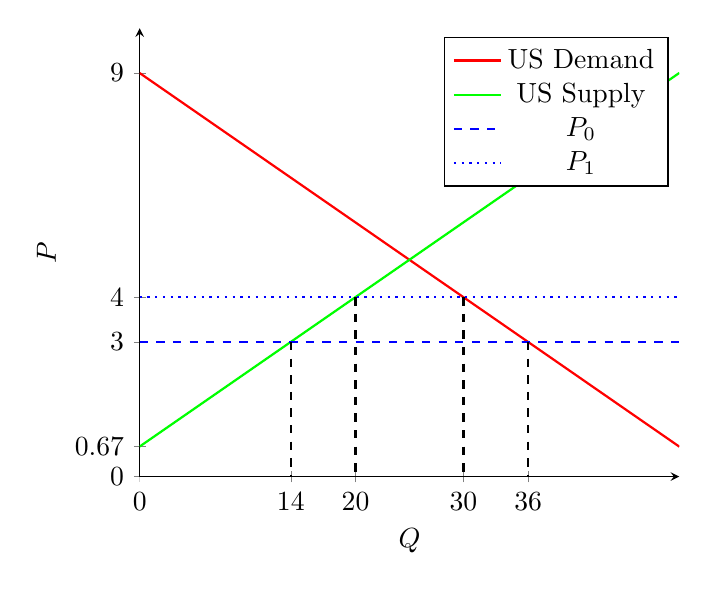
\begin{tikzpicture}
        \begin{axis}[
            axis lines = left,
            xlabel = $Q$,
            ylabel = $P$,
            ymax = 10,
            ymin = 0,
            xmax = 50,
            xmin = 0,
            scaled x ticks = false,
            ytick = {0,.67, 3,4,9},
            xtick = {0,14,20,30,36}
        ]
        \addplot[
        color=red,thick,
        domain=0:50,
        range = 0:50]{-x/6 + 9};
        \addlegendentry{US Demand}
        \addplot[
        color=green,thick,
        domain=0:50,
        range = 0:50]{x/6 + .67};
        \addlegendentry{US Supply}
        \addplot[
        color=blue,thick,dashed,
        domain=0:50,
        range = 0:50]{3};
        \addlegendentry{{$P_0$}}
        \addplot[
        color=blue,thick,dotted,
        domain=0:50,
        range = 0:50]{4};
        \addlegendentry{{$P_1$}}
        % \addplot[
        % black,thick,dashed]
        % coordinates {
        %     (12,0)
        %     (12,3)
        %     (0,3)
        % };
        \addplot[
        black,thick,dashed]
        coordinates {
            (14,3)
            (14,0)
        };
        \addplot[
        black,thick,dashed]
        coordinates {
            (20,4)
            (20,0)
        };
        \addplot[
        black,thick,dashed]
        coordinates {
            (30,4)
            (30,0)
        };
        \addplot[
        black,thick,dashed]
        coordinates {
            (36,3)
            (36,0)
        };
        \end{axis}
        \end{tikzpicture}
    \end{center}
\end{frame}

\begin{frame}{Bragabong}
    If there is no quota how many kilos of almonds would domestic producers supply and what quantity would be imported?
    \begin{center}
        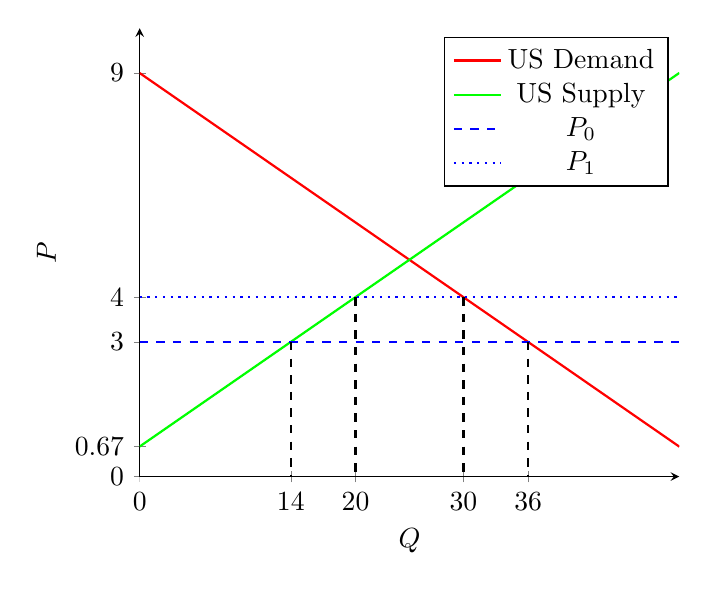
\begin{tikzpicture}
        \begin{axis}[
            axis lines = left,
            xlabel = $Q$,
            ylabel = $P$,
            ymax = 10,
            ymin = 0,
            xmax = 50,
            xmin = 0,
            scaled x ticks = false,
            ytick = {0,.67, 3,4,9},
            xtick = {0,14,20,30,36}
        ]
        \addplot[
        color=red,thick,
        domain=0:50,
        range = 0:50]{-x/6 + 9};
        \addlegendentry{US Demand}
        \addplot[
        color=green,thick,
        domain=0:50,
        range = 0:50]{x/6 + .67};
        \addlegendentry{US Supply}
        \addplot[
        color=blue,thick,dashed,
        domain=0:50,
        range = 0:50]{3};
        \addlegendentry{{$P_0$}}
        \addplot[
        color=blue,thick,dotted,
        domain=0:50,
        range = 0:50]{4};
        \addlegendentry{{$P_1$}}
        % \addplot[
        % black,thick,dashed]
        % coordinates {
        %     (12,0)
        %     (12,3)
        %     (0,3)
        % };
        \addplot[
        black,thick,dashed]
        coordinates {
            (14,3)
            (14,0)
        };
        \addplot[
        black,thick,dashed]
        coordinates {
            (20,4)
            (20,0)
        };
        \addplot[
        black,thick,dashed]
        coordinates {
            (30,4)
            (30,0)
        };
        \addplot[
        black,thick,dashed]
        coordinates {
            (36,3)
            (36,0)
        };
        \end{axis}
        \end{tikzpicture}
    \end{center}
\end{frame}

\begin{frame}{Bragabong}
    If there is no quota what is the dollar value of consumer surplus?
    \begin{center}
        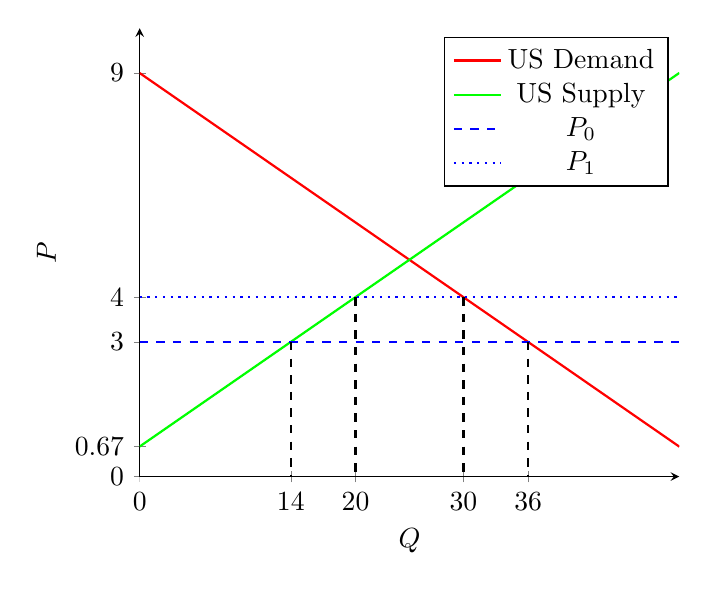
\begin{tikzpicture}
        \begin{axis}[
            axis lines = left,
            xlabel = $Q$,
            ylabel = $P$,
            ymax = 10,
            ymin = 0,
            xmax = 50,
            xmin = 0,
            scaled x ticks = false,
            ytick = {0,.67, 3,4,9},
            xtick = {0,14,20,30,36}
        ]
        \addplot[
        color=red,thick,
        domain=0:50,
        range = 0:50]{-x/6 + 9};
        \addlegendentry{US Demand}
        \addplot[
        color=green,thick,
        domain=0:50,
        range = 0:50]{x/6 + .67};
        \addlegendentry{US Supply}
        \addplot[
        color=blue,thick,dashed,
        domain=0:50,
        range = 0:50]{3};
        \addlegendentry{{$P_0$}}
        \addplot[
        color=blue,thick,dotted,
        domain=0:50,
        range = 0:50]{4};
        \addlegendentry{{$P_1$}}
        % \addplot[
        % black,thick,dashed]
        % coordinates {
        %     (12,0)
        %     (12,3)
        %     (0,3)
        % };
        \addplot[
        black,thick,dashed]
        coordinates {
            (14,3)
            (14,0)
        };
        \addplot[
        black,thick,dashed]
        coordinates {
            (20,4)
            (20,0)
        };
        \addplot[
        black,thick,dashed]
        coordinates {
            (30,4)
            (30,0)
        };
        \addplot[
        black,thick,dashed]
        coordinates {
            (36,3)
            (36,0)
        };
        \end{axis}
        \end{tikzpicture}
    \end{center}
\end{frame}

\begin{frame}[t]{Bragabong}
    \textbf{If there is no quota what is the dollar value of consumer surplus?}
    \newline
    \newline We simply compute the area of the triangle befor ethe quota:
    \[\begin{split}
        CS_{pre} &= \frac{(\$9-\$3)36}{2} \\
        &= \frac{(\$6)36}{2} \\
        &= \boxed{\$108} \\
    \end{split}\]
\end{frame}

\begin{frame}{Bragabong}
    If there is no quota what is the dollar value of producer surplus received by producers in Bragabong?
    \begin{center}
        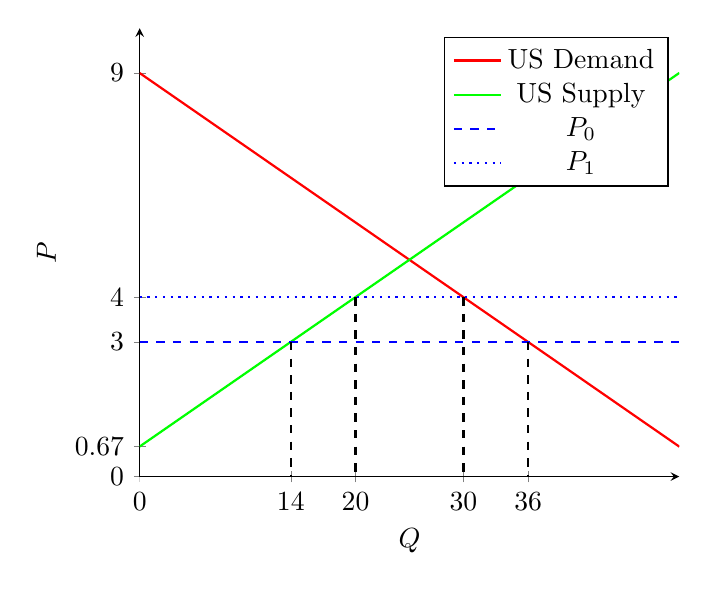
\begin{tikzpicture}
        \begin{axis}[
            axis lines = left,
            xlabel = $Q$,
            ylabel = $P$,
            ymax = 10,
            ymin = 0,
            xmax = 50,
            xmin = 0,
            scaled x ticks = false,
            ytick = {0,.67, 3,4,9},
            xtick = {0,14,20,30,36}
        ]
        \addplot[
        color=red,thick,
        domain=0:50,
        range = 0:50]{-x/6 + 9};
        \addlegendentry{US Demand}
        \addplot[
        color=green,thick,
        domain=0:50,
        range = 0:50]{x/6 + .67};
        \addlegendentry{US Supply}
        \addplot[
        color=blue,thick,dashed,
        domain=0:50,
        range = 0:50]{3};
        \addlegendentry{{$P_0$}}
        \addplot[
        color=blue,thick,dotted,
        domain=0:50,
        range = 0:50]{4};
        \addlegendentry{{$P_1$}}
        % \addplot[
        % black,thick,dashed]
        % coordinates {
        %     (12,0)
        %     (12,3)
        %     (0,3)
        % };
        \addplot[
        black,thick,dashed]
        coordinates {
            (14,3)
            (14,0)
        };
        \addplot[
        black,thick,dashed]
        coordinates {
            (20,4)
            (20,0)
        };
        \addplot[
        black,thick,dashed]
        coordinates {
            (30,4)
            (30,0)
        };
        \addplot[
        black,thick,dashed]
        coordinates {
            (36,3)
            (36,0)
        };
        \end{axis}
        \end{tikzpicture}
    \end{center}
\end{frame}

\begin{frame}{Bragabong}
    \textbf{If there is no quota, what is the dollar value of producer surplus received by producers in Bragabong?}
    \newline
    \newline Compute producer surplus at $P_0$:
    \[\begin{split}
        PS_{pre} &= \frac{(\$3-\$.67)14}{2} \\
        &= \frac{(\$2.33)14}{2} \\
        &= \boxed{\$16.31}
    \end{split}\]
\end{frame}

\begin{frame}{Bragabong}
    If there is no quota what is the revenue received by foreign producers who supply almonds to Bragabong?
    \begin{center}
        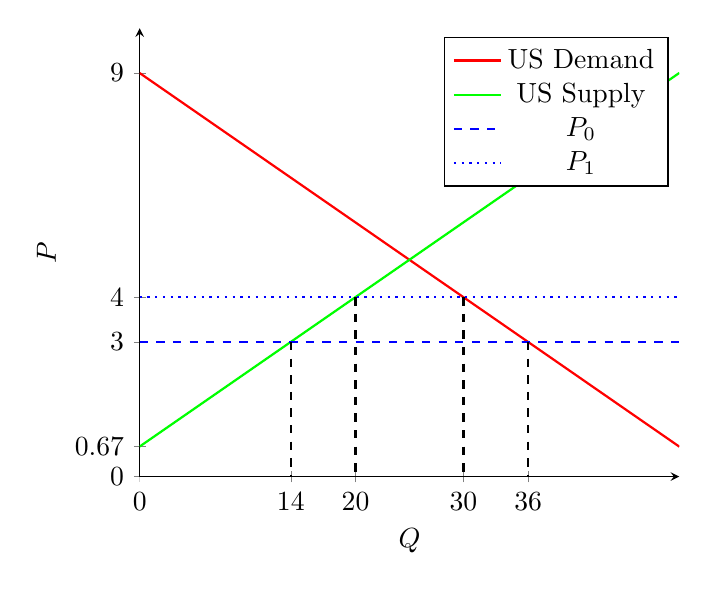
\begin{tikzpicture}
        \begin{axis}[
            axis lines = left,
            xlabel = $Q$,
            ylabel = $P$,
            ymax = 10,
            ymin = 0,
            xmax = 50,
            xmin = 0,
            scaled x ticks = false,
            ytick = {0,.67, 3,4,9},
            xtick = {0,14,20,30,36}
        ]
        \addplot[
        color=red,thick,
        domain=0:50,
        range = 0:50]{-x/6 + 9};
        \addlegendentry{US Demand}
        \addplot[
        color=green,thick,
        domain=0:50,
        range = 0:50]{x/6 + .67};
        \addlegendentry{US Supply}
        \addplot[
        color=blue,thick,dashed,
        domain=0:50,
        range = 0:50]{3};
        \addlegendentry{{$P_0$}}
        \addplot[
        color=blue,thick,dotted,
        domain=0:50,
        range = 0:50]{4};
        \addlegendentry{{$P_1$}}
        % \addplot[
        % black,thick,dashed]
        % coordinates {
        %     (12,0)
        %     (12,3)
        %     (0,3)
        % };
        \addplot[
        black,thick,dashed]
        coordinates {
            (14,3)
            (14,0)
        };
        \addplot[
        black,thick,dashed]
        coordinates {
            (20,4)
            (20,0)
        };
        \addplot[
        black,thick,dashed]
        coordinates {
            (30,4)
            (30,0)
        };
        \addplot[
        black,thick,dashed]
        coordinates {
            (36,3)
            (36,0)
        };
        \end{axis}
        \end{tikzpicture}
    \end{center}
\end{frame}

\begin{frame}[t]{Bragabong}
    \textbf{If there is no quota what is the revenue received by foreign producers who supply almonds to Bragabong?} 
    \newline
    \newline We simply calculate the quantity supplied at $P_0$:
    \[\text{Foreign Producer Revenue} = (36-14) \times \$3 = \boxed{\$66}\]
\end{frame}

\begin{frame}{Bragabong}
    With a quota in place what is the price that consumers of Bragabong must now pay and what is the quantity demanded?
    \begin{center}
        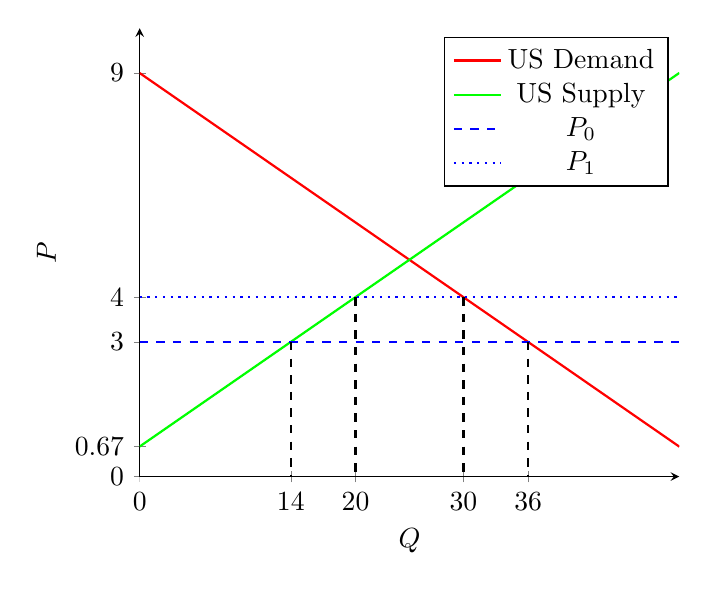
\begin{tikzpicture}
        \begin{axis}[
            axis lines = left,
            xlabel = $Q$,
            ylabel = $P$,
            ymax = 10,
            ymin = 0,
            xmax = 50,
            xmin = 0,
            scaled x ticks = false,
            ytick = {0,.67, 3,4,9},
            xtick = {0,14,20,30,36}
        ]
        \addplot[
        color=red,thick,
        domain=0:50,
        range = 0:50]{-x/6 + 9};
        \addlegendentry{US Demand}
        \addplot[
        color=green,thick,
        domain=0:50,
        range = 0:50]{x/6 + .67};
        \addlegendentry{US Supply}
        \addplot[
        color=blue,thick,dashed,
        domain=0:50,
        range = 0:50]{3};
        \addlegendentry{{$P_0$}}
        \addplot[
        color=blue,thick,dotted,
        domain=0:50,
        range = 0:50]{4};
        \addlegendentry{{$P_1$}}
        % \addplot[
        % black,thick,dashed]
        % coordinates {
        %     (12,0)
        %     (12,3)
        %     (0,3)
        % };
        \addplot[
        black,thick,dashed]
        coordinates {
            (14,3)
            (14,0)
        };
        \addplot[
        black,thick,dashed]
        coordinates {
            (20,4)
            (20,0)
        };
        \addplot[
        black,thick,dashed]
        coordinates {
            (30,4)
            (30,0)
        };
        \addplot[
        black,thick,dashed]
        coordinates {
            (36,3)
            (36,0)
        };
        \end{axis}
        \end{tikzpicture}
    \end{center}
\end{frame}

\begin{frame}{Bragabong}
    With a quota in place what is the dollar value of consumer surplus? Are consumers better off?
    \begin{center}
        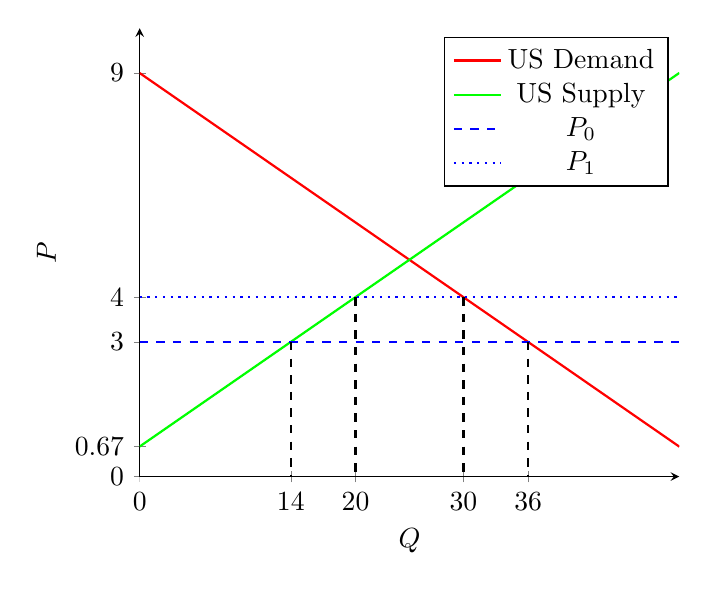
\begin{tikzpicture}
        \begin{axis}[
            axis lines = left,
            xlabel = $Q$,
            ylabel = $P$,
            ymax = 10,
            ymin = 0,
            xmax = 50,
            xmin = 0,
            scaled x ticks = false,
            ytick = {0,.67, 3,4,9},
            xtick = {0,14,20,30,36}
        ]
        \addplot[
        color=red,thick,
        domain=0:50,
        range = 0:50]{-x/6 + 9};
        \addlegendentry{US Demand}
        \addplot[
        color=green,thick,
        domain=0:50,
        range = 0:50]{x/6 + .67};
        \addlegendentry{US Supply}
        \addplot[
        color=blue,thick,dashed,
        domain=0:50,
        range = 0:50]{3};
        \addlegendentry{{$P_0$}}
        \addplot[
        color=blue,thick,dotted,
        domain=0:50,
        range = 0:50]{4};
        \addlegendentry{{$P_1$}}
        % \addplot[
        % black,thick,dashed]
        % coordinates {
        %     (12,0)
        %     (12,3)
        %     (0,3)
        % };
        \addplot[
        black,thick,dashed]
        coordinates {
            (14,3)
            (14,0)
        };
        \addplot[
        black,thick,dashed]
        coordinates {
            (20,4)
            (20,0)
        };
        \addplot[
        black,thick,dashed]
        coordinates {
            (30,4)
            (30,0)
        };
        \addplot[
        black,thick,dashed]
        coordinates {
            (36,3)
            (36,0)
        };
        \end{axis}
        \end{tikzpicture}
    \end{center}
\end{frame}

\begin{frame}[t]{Bragabong}
    \textbf{With a quota in place what is the dollar value of consumer surplus? Are consumers better off?} 
    \newline
    \newline We calculate consumer surplus at $P_1$:
    \[\begin{split}
        CS_{post} &= \frac{(\$9-\$4)30}{2} \\
        &= \frac{(\$5)30}{2} \\
        &= \boxed{\$75}
    \end{split}\]
    So consumers are worse off, as before the quota, they had \$108 of consumer surplus.
\end{frame}

\begin{frame}{Bragabong}
    With a quota in place what is the dollar value of producer surplus received by producers in Bragabong? Are domestic producers better off?
    \begin{center}
        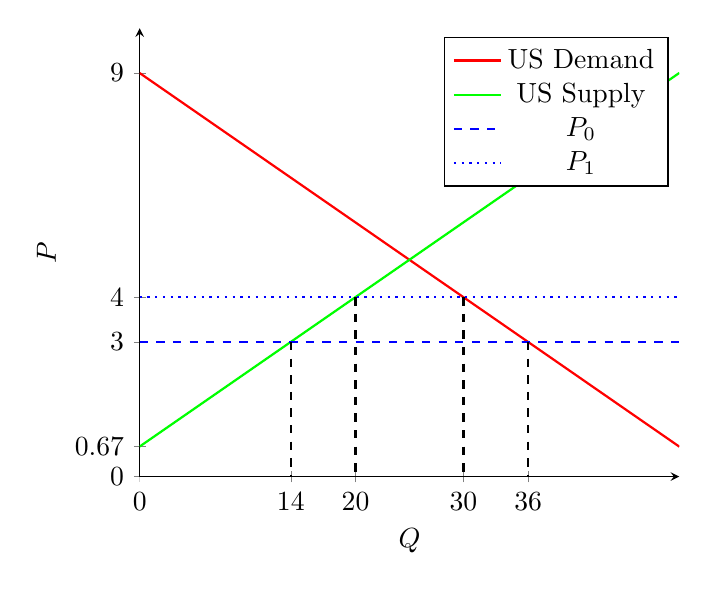
\begin{tikzpicture}
        \begin{axis}[
            axis lines = left,
            xlabel = $Q$,
            ylabel = $P$,
            ymax = 10,
            ymin = 0,
            xmax = 50,
            xmin = 0,
            scaled x ticks = false,
            ytick = {0,.67, 3,4,9},
            xtick = {0,14,20,30,36}
        ]
        \addplot[
        color=red,thick,
        domain=0:50,
        range = 0:50]{-x/6 + 9};
        \addlegendentry{US Demand}
        \addplot[
        color=green,thick,
        domain=0:50,
        range = 0:50]{x/6 + .67};
        \addlegendentry{US Supply}
        \addplot[
        color=blue,thick,dashed,
        domain=0:50,
        range = 0:50]{3};
        \addlegendentry{{$P_0$}}
        \addplot[
        color=blue,thick,dotted,
        domain=0:50,
        range = 0:50]{4};
        \addlegendentry{{$P_1$}}
        % \addplot[
        % black,thick,dashed]
        % coordinates {
        %     (12,0)
        %     (12,3)
        %     (0,3)
        % };
        \addplot[
        black,thick,dashed]
        coordinates {
            (14,3)
            (14,0)
        };
        \addplot[
        black,thick,dashed]
        coordinates {
            (20,4)
            (20,0)
        };
        \addplot[
        black,thick,dashed]
        coordinates {
            (30,4)
            (30,0)
        };
        \addplot[
        black,thick,dashed]
        coordinates {
            (36,3)
            (36,0)
        };
        \end{axis}
        \end{tikzpicture}
    \end{center}
\end{frame}

\begin{frame}[t]{Bragabong}
    \textbf{With a quota in place what is the dollar value of producer surplus received by producers in Bragabong? Are domestic producers better off?}
    \newline
    \newline We calculate producer surplus at $P_1$:
    \[\begin{split}
        PS_{post} &= \frac{(\$4-\$.67)20}{2} \\
        &= \frac{(\$3.33)20}{2} \\
        &= \boxed{\$33.3}
    \end{split}\]
    As domestic producers received only \$16.31 before the quota, they are better off.
\end{frame}

\begin{frame}{Bragabong}
    Calculate the revenue to foreign producers who are granted permission to sell in Bragabong after the imposition of the quota.
    \begin{center}
        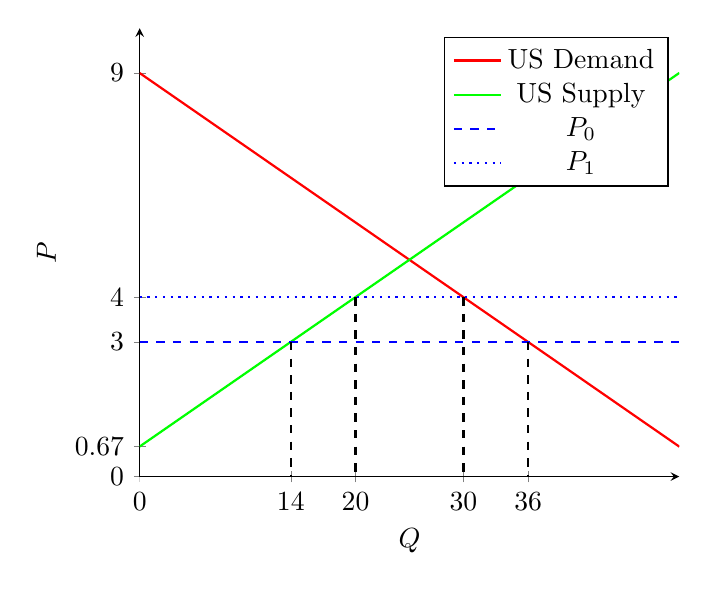
\begin{tikzpicture}
        \begin{axis}[
            axis lines = left,
            xlabel = $Q$,
            ylabel = $P$,
            ymax = 10,
            ymin = 0,
            xmax = 50,
            xmin = 0,
            scaled x ticks = false,
            ytick = {0,.67, 3,4,9},
            xtick = {0,14,20,30,36}
        ]
        \addplot[
        color=red,thick,
        domain=0:50,
        range = 0:50]{-x/6 + 9};
        \addlegendentry{US Demand}
        \addplot[
        color=green,thick,
        domain=0:50,
        range = 0:50]{x/6 + .67};
        \addlegendentry{US Supply}
        \addplot[
        color=blue,thick,dashed,
        domain=0:50,
        range = 0:50]{3};
        \addlegendentry{{$P_0$}}
        \addplot[
        color=blue,thick,dotted,
        domain=0:50,
        range = 0:50]{4};
        \addlegendentry{{$P_1$}}
        % \addplot[
        % black,thick,dashed]
        % coordinates {
        %     (12,0)
        %     (12,3)
        %     (0,3)
        % };
        \addplot[
        black,thick,dashed]
        coordinates {
            (14,3)
            (14,0)
        };
        \addplot[
        black,thick,dashed]
        coordinates {
            (20,4)
            (20,0)
        };
        \addplot[
        black,thick,dashed]
        coordinates {
            (30,4)
            (30,0)
        };
        \addplot[
        black,thick,dashed]
        coordinates {
            (36,3)
            (36,0)
        };
        \end{axis}
        \end{tikzpicture}
    \end{center}
\end{frame}

\begin{frame}[t]{Bragabong}
    \textbf{Calculate the revenue to foreign producers who are granted permission to sell in Bragabong after the imposition of the quota.}
    \newline
    \newline We know that they can only produce 10 units, and they produce at $P_1 = \$4$, so we have
    \[\text{Foreign Producer Revenue} = \$4 \times 10 = \boxed{\$40}\]
\end{frame}

\begin{frame}{Bragabong}
    Calculate the deadweight loss as a result of the quota.
    \begin{center}
        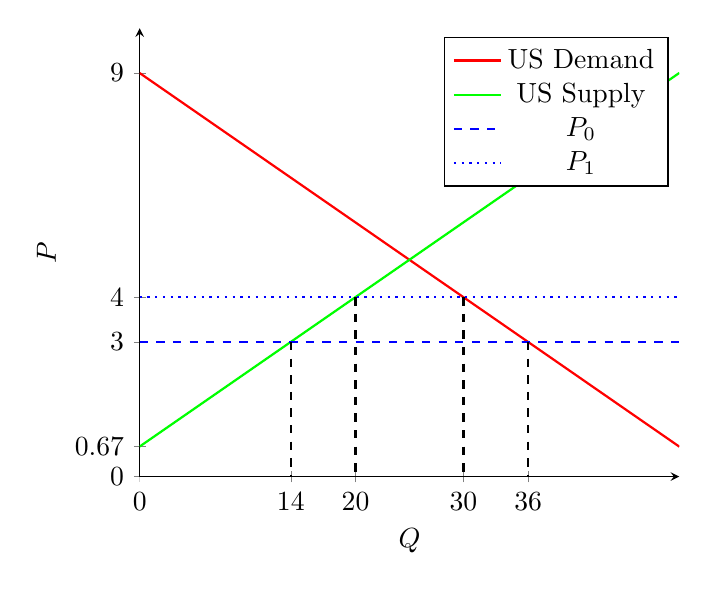
\begin{tikzpicture}
        \begin{axis}[
            axis lines = left,
            xlabel = $Q$,
            ylabel = $P$,
            ymax = 10,
            ymin = 0,
            xmax = 50,
            xmin = 0,
            scaled x ticks = false,
            ytick = {0,.67, 3,4,9},
            xtick = {0,14,20,30,36}
        ]
        \addplot[
        color=red,thick,
        domain=0:50,
        range = 0:50]{-x/6 + 9};
        \addlegendentry{US Demand}
        \addplot[
        color=green,thick,
        domain=0:50,
        range = 0:50]{x/6 + .67};
        \addlegendentry{US Supply}
        \addplot[
        color=blue,thick,dashed,
        domain=0:50,
        range = 0:50]{3};
        \addlegendentry{{$P_0$}}
        \addplot[
        color=blue,thick,dotted,
        domain=0:50,
        range = 0:50]{4};
        \addlegendentry{{$P_1$}}
        % \addplot[
        % black,thick,dashed]
        % coordinates {
        %     (12,0)
        %     (12,3)
        %     (0,3)
        % };
        \addplot[
        black,thick,dashed]
        coordinates {
            (14,3)
            (14,0)
        };
        \addplot[
        black,thick,dashed]
        coordinates {
            (20,4)
            (20,0)
        };
        \addplot[
        black,thick,dashed]
        coordinates {
            (30,4)
            (30,0)
        };
        \addplot[
        black,thick,dashed]
        coordinates {
            (36,3)
            (36,0)
        };
        \end{axis}
        \end{tikzpicture}
    \end{center}
\end{frame}

\begin{frame}[t]{Bragabong}
    \textbf{Calculate the deadweight loss as a result of the quota.}
    \newline
    \newline The deadweight loss will be the surplus that is eliminated as a result of the tariff:
    \[\begin{split}
        DWL &= \frac{(\$4-\$3)(20-14)}{2} + \frac{(\$4-\$3)(36-30)}{2} \\
        &= \frac{(\$1)(6)}{2} + \frac{(\$1)(6)}{2} \\
        &= \boxed{\$6}
    \end{split}\]
\end{frame}

\begin{frame}{Externalities}
    \begin{itemize}
        \item What is an externality?
        \begin{itemize}
            \item A benefit or cost generated by an activity that affects an economic agent not directly involved in the activity
        \end{itemize}
        \item What is market failure?
        \begin{itemize}
            \item A market failure refers to the inability of the market to allocate resources efficiently up to the point where marginal social benefit equals marginal social cost.
        \end{itemize}
        \item How do externalities lead to market failures?
        \begin{itemize}
            \item Remember, deadweight loss comes from over- or under-production of a good. Externalities cause agents to not bear the full cost or benefit of their actions, which means that they do not produce optimally. Nonoptimal production implies deadweight loss.
        \end{itemize}
    \end{itemize}
\end{frame}

\begin{frame}{Joshua Tree}
    The figure shows supply and demand for planting trees, based on private costs and benefits. Trees sequester carbon, meaning that they help counteract pollutants that contribute to climate change.
    \begin{center}
        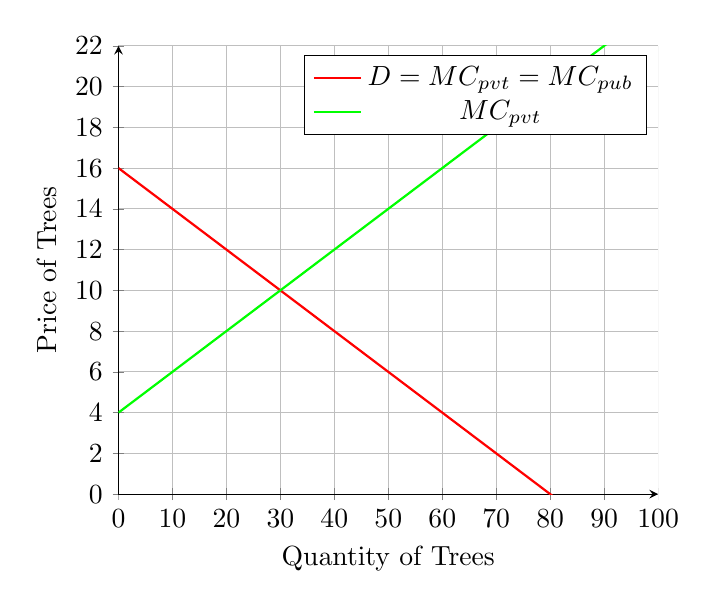
\begin{tikzpicture}
        \begin{axis}[
            axis lines = left,
            xlabel = {Quantity of Trees},
            ylabel = {Price of Trees},
            ymax = 22,
            ymin = 0,
            xmax = 100,
            xmin = 0,
            scaled x ticks = false,
            ytick distance = 2,
            xtick distance = 10,
            grid = both
        ]
        \addplot[
        color=red,thick,
        domain=0:100,
        range = 0:100]{-x/5 + 16};
        \addlegendentry{$D=MC_{pvt}=MC_{pub}$}
        \addplot[
        color=green,thick,
        domain=0:100,
        range = 0:100]{x/5 + 4};
        \addlegendentry{$MC_{pvt}$}
        \end{axis}
        \end{tikzpicture}
    \end{center}
\end{frame}

\begin{frame}[t]{Joshua Tree}
    \begin{itemize}
        \item[a.] Suppose that the carbon sequestration that results from planting a tree is worth \$4. Graph the social cost curve for tree planting that accounts for the positive externality of trees.
        \item[b.] Ignoring the positive externality, how many trees will be planted?
        \item[c.] What is the socially optimal quantity of trees?
        \item[d.] What is the deadweight loss that occurs when suppliers are unable to capture the \$4 external benefit they provide from planting trees? Graph the deadweight loss.
        \item[e.] How much should the government subsidize tree planting to bring about the socially efficient level of tree planting?
    \end{itemize}
\end{frame}

\begin{frame}{Joshua Tree}
    \begin{center}
        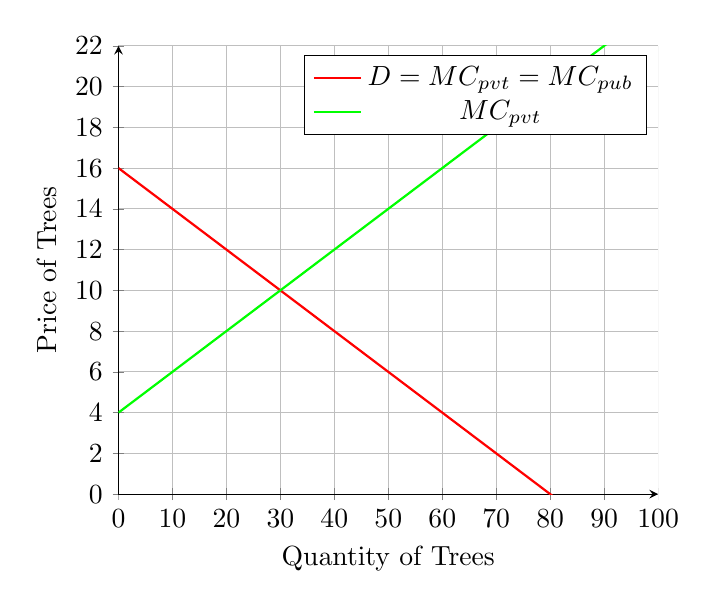
\begin{tikzpicture}
        \begin{axis}[
            axis lines = left,
            xlabel = {Quantity of Trees},
            ylabel = {Price of Trees},
            ymax = 22,
            ymin = 0,
            xmax = 100,
            xmin = 0,
            scaled x ticks = false,
            ytick distance = 2,
            xtick distance = 10,
            grid = both
        ]
        \addplot[
        color=red,thick,
        domain=0:100,
        range = 0:100]{-x/5 + 16};
        \addlegendentry{$D=MC_{pvt}=MC_{pub}$}
        \addplot[
        color=green,thick,
        domain=0:100,
        range = 0:100]{x/5 + 4};
        \addlegendentry{$MC_{pvt}$}
        \end{axis}
        \end{tikzpicture}
    \end{center}
\end{frame}

\begin{frame}{Keep the Wolves Away}
    When U.S. farmers in the Southwest irrigate their land, salt in the ground soil leaks into the Colorado River. The Colorado River has become so salty that Mexican farmers further down the river cannot irrigate their own land, and Mexican crops have suffered. Explain why this situation constitutes a negative production externality, how it leads to too much irrigation, and what it would mean for U.S. farmers to face the externality. (Draw a P-Q graph showing the negative externality, over-consumption, and DWL here)
\end{frame}

\begin{frame}{Trash}
    The city of Seattle limits each household to one can of free garbage collection per week. There are fees for any extra garbage collected from the curb. Suppose that a neighborhood group in Seattle organizes a group of families so that those who plan to go over their one-can garbage quota can find households that are under their quota and pay them to put out the extra trash. Does this change the efficiency of the policy?
\end{frame}

\begin{frame}{Keep the Wolves Away}
    The following figure shows the demand curve for a U.S. farmer for irrigating his land. It costs the farmer \$100 per acre to irrigate the land. Each acre of land irrigation generates salty runoff that winds up in the Colorado River. It costs \$50 to desalinate this river water so Mexican farmers can irrigate their crops. 
    \begin{itemize}
        \item[a.] Draw the marginal private cost of irrigation on the graph
        \item[b.] Draw the marginal social cost of irrigation on the graph
        \item[c.] How many acres will the U.S. farmer irrigate?
        \item[d.] What is the efficient level of irrigation?
    \end{itemize}
\end{frame}

\begin{frame}{Keep the Wolves Away}
    \begin{center}
        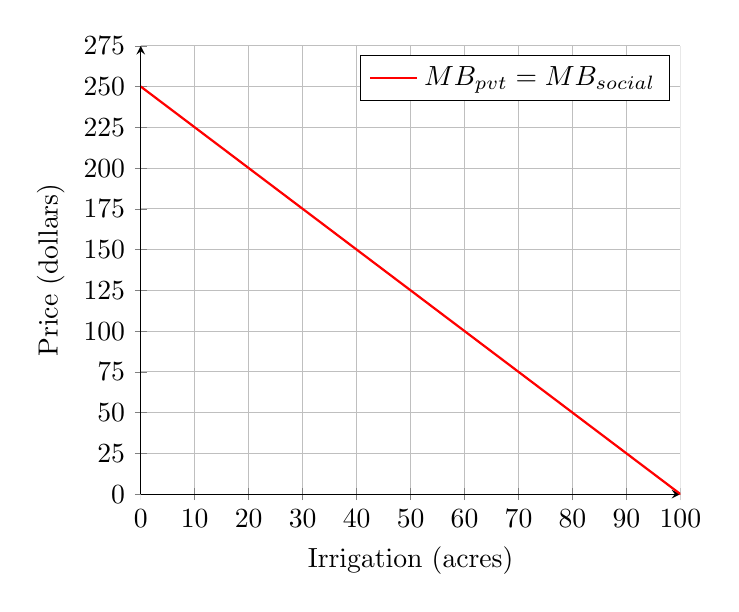
\begin{tikzpicture}
        \begin{axis}[
            axis lines = left,
            xlabel = Irrigation (acres),
            ylabel = Price (dollars),
            ymax = 275,
            ymin = 0,
            xmax = 100,
            xmin = 0,
            grid=both,
            scaled x ticks = false,
            ytick distance = 25,
            xtick distance = 10
        ]
        \addplot[
        color=red,thick,
        domain=0:300,
        range = 0:300]{-2.5*x + 250};
        \addlegendentry{{$MB_{pvt} = MB_{social}$}}
        \end{axis}
        \end{tikzpicture}
    \end{center}
\end{frame}

\begin{frame}{Coase Theorem}
    Your neighbor never mows her lawn. You don’t have any legal right to force her to mow, but the mess in her front yard is making your neighborhood unsightly and reducing the value of your house. The reduction in the value of your house is \$5,000, and the value of her time to mow the lawn once a week is \$1,000. Suppose you offer her a deal in which you pay her \$3,000 to mow. How does this deal affect surplus?
    \begin{itemize}
        \item The deal increases only your surplus.
        \item The deal increases only your neighbor’s surplus.
        \item The deal increases both your surplus and your neighbor’s.
        \item The deal increases your surplus but decreases your neighbor’s.
        \item The deal increases your neighbor’s surplus but decreases yours.
        \item The deal does not affect surplus.
    \end{itemize}
\end{frame}

\begin{frame}{Nose on the Grindstone}
    Without regulation, there are 4 coal burning power plants producing 4,000 tons of pollution per year. Economists have determined that the socially optimal amount of pollution is 2,800 tons/year. The amount of pollution produced by each firm and the cost of reducing pollution for each firm is given below.
    \begin{table}[H]
    \centering
    \begin{tabular}{lcccc}
                                                  & Firm 1 & Firm 2 & Firm 3 & Firm 4 \\
    Pollution before permits                      & 1,000  & 1,000  & 1,000  & 1,000  \\ \hline
    Cost of reducing pollution \\(per ton per year) & \$50   & \$20   & \$30   & \$40  
    \end{tabular}
    \end{table}
    If the government issues each firm a non-tradable permit to produce 700 tons of pollution per year, what will be the cost of pollution reduction?
\end{frame}

\begin{frame}{Nose on the Grindstone}
    If the government issues each firm a non-tradable permit to produce 700 tons of pollution per year, what will be the cost of pollution reduction?
    \begin{table}[H]
    \centering
    \begin{tabular}{lcccc}
                                                  & Firm 1 & Firm 2 & Firm 3 & Firm 4 \\
    Pollution before permits                      & 1,000  & 1,000  & 1,000  & 1,000  \\ \hline
    Cost of reducing pollution \\(per ton per year) & \$50   & \$20   & \$30   & \$40  
    \end{tabular}
    \end{table}
    Every firm will reduce by 300, which will cost
    \[300 \times (\$50 + \$20 + \$30 + \$40) = 300 \times \$140 = \boxed{\$42,000}\]
\end{frame}

\begin{frame}{Nose on the Grindstone}
    Without regulation, there are 4 coal burning power plants producing 4,000 tons of pollution per year. Economists have determined that the socially optimal amount of pollution is 2,800 tons/year. The amount of pollution produced by each firm and the cost of reducing pollution for each firm is given below.
    \begin{table}[H]
    \centering
    \begin{tabular}{lcccc}
                                                  & Firm 1 & Firm 2 & Firm 3 & Firm 4 \\
    Pollution before permits                      & 1,000  & 1,000  & 1,000  & 1,000  \\ \hline
    Cost of reducing pollution \\(per ton per year) & \$50   & \$20   & \$30   & \$40  
    \end{tabular}
    \end{table}
    If the permits are tradable, what will be the cost of pollution reduction and what will the final amount of pollution be for each firm?
\end{frame}

\begin{frame}{Nose on the Grindstone}
    If the permits are tradable, what will be the cost of pollution reduction and what will the final amount of pollution be for each firm?
    \begin{table}[H]
    \centering
    \begin{tabular}{lcccc}
                                                  & Firm 1 & Firm 2 & Firm 3 & Firm 4 \\
    Pollution before permits                      & 1,000  & 1,000  & 1,000  & 1,000  \\ \hline
    Cost of reducing pollution \\(per ton per year) & \$50   & \$20   & \$30   & \$40  
    \end{tabular}
    \end{table}
    Since they can trade permits, and all have differential costs to reducing pollution, the lower cost reducers (Firm 2 and Firm 3) can trade their permits to the higher cost reducers (Firm 1 and Firm 4). To remove 1,200 tons of pollution, Firm 2 will remove all of their pollution (lowest cost) and Firm 2 will remove the remaining 200 tons (next lowest cost). The cost of this reduction is 
    \[1,000 \times \$20 + 200 \times \$30 = \$20,000 + \$6,000 = \$26,000\]
    Note that this assumes that trade occurs at the firm's cost of reducing pollution (which is to say that Firm 2 and Firm 3 do not profit from this transaction).
\end{frame}
% \begin{frame}{Elasticity}
%     \begin{itemize}
%         \item Price elasticity of demand describes the size of the change in the quantity demanded of a good or service when its price changes.
%         \begin{itemize}
%             \item When consumers’ buying decisions are highly influenced by price, we say that their demand is \textit{more elastic}.
%             \item When consumers are not very sensitive to price changes—that is, when they will buy approximately the same quantity, regardless of the price—we say that their demand is \textit{more inelastic}.
%         \end{itemize}
%         \item Elasticity calculation uses the midpoint formula:
%         \[\varepsilon = \frac{\frac{Q_{new} - Q_{old}}{\text{Average of $Q$}}}{\frac{P_{new} - P_{old}}{\text{Average of $P$}}} = \frac{Q_{new} - Q_{old}}{\frac{Q_{new} + Q_{old}}{2}} \frac{\frac{P_{new} + P_{old}}{2}}{P_{new} - P_{old}}\]
%         \item Price elasticity of demand is always negative (why?)
%     \end{itemize}
% \end{frame}

% \begin{frame}[t]{Determinants of PED}
%     What determines the price elasticity of demand?
% \end{frame}

% \begin{frame}[t]{Determinants of PED}
%     What determines the price elasticity of demand?
%     \begin{itemize}
%         \item Availability of substitutes
%         \item Degree of necessity
%         \item Cost relative to income
%         \item Adjustment time
%         \item Scope of the market
%     \end{itemize}
% \end{frame}

% \begin{frame}{Other Elasticities}
%     \begin{itemize}
%         \item Price elasticity of supply
%         \item Cross-price elasticity of demand
%         \item Income elasticity of demand
%     \end{itemize}
% \end{frame}

% \begin{frame}{Other Elasticities}
%     \begin{center}
%         \includegraphics[scale=.3]{table}
%     \end{center}
% \end{frame}

% \begin{frame}{Surplus}
%     \begin{itemize}
%         \item Willingness to pay: the maximum price an agent is willing to pay for a good
%         \item Willingness to sell: the minimum price an agent is willing to sell a good for
%         % \item At prices above the maximum willingness to pay for consumers, the opportunity cost is greater than the benefits. At lower prices, the benefits outweigh the opportunity cost.
%         \item Surplus is a way of measuring who benefits from transactions and by how much. 
%         \begin{itemize}
%             \item The difference between willingness to pay/sell and the actual price.
%         \end{itemize}
%     \end{itemize}
% \end{frame}

% \begin{frame}{Elasticity Calculation}
%     \begin{tikzpicture}
%     \begin{axis}[
%         axis lines = left,
%         xmin=0, xmax=6,
%         ymin=0, ymax=25,
%         xlabel = {$Q$},
%         ylabel = {$P$},
%     ]
%     \addplot[thick] {-4*x + 20};
%     \node[label={0:{A (1,16)}},circle,fill,inner sep=2pt] at (axis cs:1, 16) {};
%     \node[label={0:{B (2,12)}},circle,fill,inner sep=2pt] at (axis cs:2, 12) {};
%     \end{axis}
%     \end{tikzpicture}
% \end{frame}

% \begin{frame}{Elasticity Calculation}
%     \[\begin{split}
%         \varepsilon &= \frac{\frac{Q_{new} - Q_{old}}{(Q_{old} + Q_{new}) / 2}}{\frac{P_{new} - P_{old}}{(P_{old} + P_{new}) / 2}} \\
%         &= \frac{\frac{2-1}{1.5}}{\frac{12-16}{14}} \\
%         &= -\frac{1}{1.5}\frac{14}{4}\\
%         &= -\frac{14}{6} \\
%         &\approx -2.33
%     \end{split}\]
% \end{frame}

% \begin{frame}{Perfectly Elastic Demand}
%     \begin{center}
%         \begin{tikzpicture}
%         \begin{axis}[
%         axis lines = left,
%         xlabel = $Q$,
%         ylabel = $P$,
%         xmin = -20,
%         ymin = -20,
%         xmax = 20,
%         ymax = 20,
%         yticklabels={,,},
%         xticklabels={,,},
%         ticks = none]
%         \end{axis}
%         \end{tikzpicture}
%     \end{center}
% \end{frame}

% \begin{frame}{Perfectly Inelastic Demand}
%     \begin{center}
%         \begin{tikzpicture}
%         \begin{axis}[
%         axis lines = left,
%         xlabel = $Q$,
%         ylabel = $P$,
%         xmin = -20,
%         ymin = -20,
%         xmax = 20,
%         ymax = 20,
%         yticklabels={,,},
%         xticklabels={,,},
%         ticks = none]
%         \end{axis}
%         \end{tikzpicture}
%     \end{center}
% \end{frame}

% \begin{frame}{Relatively More/Less Elastic Demand}
%     \begin{center}
%         \begin{tikzpicture}
%         \begin{axis}[
%         axis lines = left,
%         xlabel = $Q$,
%         ylabel = $P$,
%         xmin = 0,
%         ymin = 0,
%         xmax = 20,
%         ymax = 20,
%         yticklabels={,,},
%         xticklabels={,,},
%         ticks = none]
%         \addplot[thick][domain=0:20]{-1.3*x + 18};
%         \end{axis}
%         \end{tikzpicture}
%     \end{center}
% \end{frame}

% \begin{frame}[t]{Chocolate}
%     When the price of a bar of chocolate is \$1.00, the quantity demanded is 100,000 bars. When the price rises to \$1.50, the quantity demanded falls to 60,000 bars. Calculate the price elasticity of demand using the mid-point method.
% \end{frame}

% \begin{frame}{Chocolate}
%     \[\begin{split}
%         \varepsilon &= \frac{\frac{60,000 - 100,000}{80,000}}{\frac{1.50 - 1.00}{1.25}} \\
%         &= -\frac{.5}{\frac{.5}{1.25}} \\
%         &= \boxed{-1.25}
%     \end{split}\]
% \end{frame}

% \begin{frame}[t]{Chocolate}
%     When the price of a bar of chocolate is \$1.00, the quantity demanded is 100,000 bars. When the price rises to \$1.50, the quantity demanded falls to 60,000 bars. What is the price effect and quantity effect for this change? What happens to total revenue?
% \end{frame}

% \begin{frame}{Chocolate}
%     Price Effect:
%     \[\$0.50 \times 60,000 = \$30,000\]
%     Quantity Effect:
%     \[\$1 \times -40,000 = -\$40,000\]
%     Change in Total Revenue
%     \[\$30,000 - \$40,000 = -\$10,000\]
% \end{frame}

% \begin{frame}[t]{Used Cars}
%     If the price elasticity of demand for used cars priced between \$3,000 and \$5,000 is –1.2 (using the mid-point method), what will be the percent change in quantity demanded when the price of a used car falls from \$5,000 to \$3,000?
% \end{frame}

% \begin{frame}{Used Cars}
%     \[\begin{split}
%         -1.2 &= \frac{\text{\% Change in Quantity Demanded}}{\frac{3,000 - 5,000}{4,000}} \\
%         &=\frac{\text{\% Change in Quantity Demanded}}{\frac{-2,000}{4,000}} \\
%         &=\frac{\text{\% Change in Quantity Demanded}}{-.5} \\
%         \implies .6 &= \text{\% Change in Quantity Demanded} \\
%         \implies \boxed{60\%} &= \text{\% Change in Quantity Demanded} 
%     \end{split}\]
% \end{frame}

% \begin{frame}[t]{Short-Run Elasticity}
%     Which of the following has a more elastic demand in the short run?
% \end{frame}

% \begin{frame}[t]{Short-Run Elasticity}
%     Which of the following has a more elastic demand in the short run?
%     \begin{itemize}
%         \item Pomegranate juice or drinking water?
%         \item Cereal or Rice Krispies®?
%         \item Speedboats or gourmet chocolate?
%     \end{itemize}
% \end{frame}

% \begin{frame}[t]{Short-Run Elasticity}
%     Which of the following has a more elastic demand in the short run?
%     \begin{itemize}
%         \item \textbf{Pomegranate juice} or drinking water?
%         \item Cereal or \textbf{Rice Krispies®}?
%         \item \textbf{Speedboats} or gourmet chocolate?
%     \end{itemize}
% \end{frame}

% \begin{frame}{Surplus}
%     \begin{itemize}
%         \item What is marginal benefit?
%         \item Why is the demand curve referred to as the marginal benefit curve?
%         \item What is marginal cost?
%         \item Why is the supply curve referred to as the marginal cost curve?
%     \end{itemize}
% \end{frame}

% \begin{frame}[t]{Mona Lisa}
%     Suppose you are offered the chance to purchase the Mona Lisa for \$5 million, but you consider this painting to be (without any exaggeration) ``priceless". What is your consumer surplus?
% \end{frame}

% \begin{frame}[t]{Oranges}
%     Suppose the market for oranges looks like this:
%     \begin{center}
%         \begin{tikzpicture}
%         \begin{axis}[
%             axis lines = left,
%             xlabel = $Q$,
%             ylabel = $P$,
%             ymax = 50,
%             ymin = 0,
%             xmax = 50,
%             xmin = 0,
%             scaled x ticks = false,
%             ytick = {0,5,10,15,20,25,30,35,40,45,50}
%         ]
%         % \addplot [color=blue,fill=blue, 
%         %                     fill opacity=0.05]
%         %                     coordinates {
%         %             (0, 20) 
%         %             (0, 23)
%         %             (6, 20)  };
%         % \addplot [color=green,fill=green, 
%         %         fill opacity=0.05]
%         %         coordinates {
%         %             (0, 14) 
%         %             (0, 20)
%         %             (6,20)};
%         \addplot[
%         color=red,
%         domain=0:50,
%         range = 0:50]{-x + 45};
%         \addplot[
%         color=green,
%         domain=0:50,
%         range = 0:50]{10 + x/2};
%         % \addplot[
%         % color=black,
%         % domain=0:6,
%         % range = 0:6]{20};
%         \end{axis}
%         \end{tikzpicture}
%     \end{center}
% \end{frame}

% \begin{frame}[t]{Oranges}
%     A frost occurs, which destroys some of the orange crop. This shifts the supply curve left:
%     \begin{center}
%         \begin{tikzpicture}
%         \begin{axis}[
%             axis lines = left,
%             xlabel = $Q$,
%             ylabel = $P$,
%             ymax = 50,
%             ymin = 0,
%             xmax = 50,
%             xmin = 0,
%             scaled x ticks = false,
%             ytick = {0,5,10,15,20,25,30,35,40,45,50}
%         ]
%         % \addplot [color=blue,fill=blue, 
%         %                     fill opacity=0.05]
%         %                     coordinates {
%         %             (0, 20) 
%         %             (0, 23)
%         %             (6, 20)  };
%         % \addplot [color=green,fill=green, 
%         %         fill opacity=0.05]
%         %         coordinates {
%         %             (0, 14) 
%         %             (0, 20)
%         %             (6,20)};
%         \addplot[
%         color=red,
%         domain=0:50,
%         range = 0:50]{-x + 45};
%         \addplot[
%         color=green,
%         domain=0:50,
%         range = 0:50]{10 + x/2};
%         \addplot[
%         color=green,
%         domain=0:50,
%         range = 0:50]{20 + x/2};
%         \draw [->] (axis cs:10, 15) -- (axis cs:6, 23);
%         \draw [->] (axis cs:20, 20) -- (axis cs:16, 28);
%         \draw [->] (axis cs:30, 25) -- (axis cs:26, 33);
%         \draw [->] (axis cs:40, 30) -- (axis cs:36, 38);
%         % \addplot[
%         % color=black,
%         % domain=0:6,
%         % range = 0:6]{20};
%         \end{axis}
%         \end{tikzpicture}
%     \end{center}
% \end{frame}

% \begin{frame}[t]{Oranges}
%     Before the shift, the surplus allocations look like this:
%     \begin{center}
%         \begin{tikzpicture}
%         \begin{axis}[
%             axis lines = left,
%             xlabel = $Q$,
%             ylabel = $P$,
%             ymax = 50,
%             ymin = 0,
%             xmax = 50,
%             xmin = 0,
%             scaled x ticks = false,
%             ytick = {0,5,10,15,20,25,30,35,40,45,50}
%         ]
%         \addplot [color=blue,fill=blue, 
%                             fill opacity=0.05]
%                             coordinates {
%                     (0, 10) 
%                     (0, 65/3)
%                     (70/3, 65/3)  };
%         \addplot [color=green,fill=green, 
%                 fill opacity=0.05]
%                 coordinates {
%                     (0, 65/3) 
%                     (70/3, 65/3)
%                     (0,45)};
%         \addplot[
%         color=red,
%         domain=0:50,
%         range = 0:50]{-x + 45};
%         \addplot[
%         color=green,
%         domain=0:50,
%         range = 0:50]{10 + x/2};
%         \addplot[
%         color=green,
%         domain=0:50,
%         range = 0:50]{20 + x/2};
%         \addplot[
%         color=black,
%         domain=0:23.33,
%         range = 0:23.33]{65/3};
%         \end{axis}
%         \end{tikzpicture}
%     \end{center}
% \end{frame}

% \begin{frame}[t]{Oranges}
%     After the shift, the surplus allocations look like this:
%     \begin{center}
%         \begin{tikzpicture}
%         \begin{axis}[
%             axis lines = left,
%             xlabel = $Q$,
%             ylabel = $P$,
%             ymax = 50,
%             ymin = 0,
%             xmax = 50,
%             xmin = 0,
%             scaled x ticks = false,
%             ytick = {0,5,10,15,20,25,30,35,40,45,50}
%         ]
%         \addplot [color=blue,fill=blue, 
%                             fill opacity=0.05]
%                             coordinates {
%                     (0, 20) 
%                     (0, 85/3)
%                     (50/3, 85/3)  };
%         \addplot [color=green,fill=green, 
%                 fill opacity=0.05]
%                 coordinates {
%                     (0, 85/3) 
%                     (50/3, 85/3)
%                     (0,45)};
%         \addplot[
%         color=red,
%         domain=0:50,
%         range = 0:50]{-x + 45};
%         \addplot[
%         color=green,
%         domain=0:50,
%         range = 0:50]{10 + x/2};
%         \addplot[
%         color=green,
%         domain=0:50,
%         range = 0:50]{20 + x/2};
%         \addplot[
%         color=black,
%         domain=0:50/3,
%         range = 0:50/3]{85/3};
%         \end{axis}
%         \end{tikzpicture}
%     \end{center}
% \end{frame}

% \begin{frame}{Oranges}
%     Conclusions: the shift in supply decreases overall surplus, and also decreases the surplus of producers and consumers individually. This will not always be true, however!
% \end{frame}

% \begin{frame}{UW Football}
%     The demand for football tickets at the UW is $Q_D=80,000 - 500P$ and the supply is $QS=20,000$. Calculate the equilibrium price, quantity and Consumer/Producer Surplus.
% \end{frame}

% \begin{frame}{UW Football}
%     Recall that at equilibrium, $Q_S=Q_D=Q^*$. Thus, equilibrium quantity $Q^*$ must be 20,000. Substituting this into the demand condition yields
%     \[\begin{split}
%         &20,000 = 80,000 - 500P^* \\
%         \implies &-60,000 = -500P^* \\
%         \implies &\boxed{P^* = 120}
%     \end{split}\]
% \end{frame}

% \begin{frame}[t]{UW Football}
%     To calculate surplus, we visualize the market:
%     \begin{center}
%         \begin{tikzpicture}
%         \begin{axis}[
%             axis lines = left,
%             xlabel = $Q$,
%             ylabel = $P$,
%             ymax = 200,
%             ymin = 0,
%             xmax = 80000,
%             xmin = 0,
%             scaled x ticks = false,
%             ytick = {0,20,40,60,80,100,120,140,160,180,200}
%         ]
%         % \addplot [color=blue,fill=blue, 
%         %                     fill opacity=0.05]
%         %                     coordinates {
%         %             (0, 120) 
%         %             (0, 160)
%         %             (20000, 120)  };
%         % \addlegendentry[mark=*]{Consumer Surplus}
%         % \addplot [color=green,fill=green, 
%         %         fill opacity=0.05]
%         %         coordinates {
%         %             (0, 0) 
%         %             (0, 120)
%         %             (20000, 120)
%         %             (20000, 0)};
%         \addplot[
%         color=red,
%         domain=0:80000,
%         range = 0:80000]{-x/500 + 160};
%         \draw [color = green] (200,0) -- (200, 200);
%         \addplot[
%         color=black,
%         domain=0:20000,
%         range = 0:20000]{120};
%         \end{axis}
%         \end{tikzpicture}
%     \end{center}
    
% \end{frame}

% \begin{frame}[t]{UW Football}
%     To calculate surplus, we visualize the market:
%     \begin{center}
%         \begin{tikzpicture}
%         \begin{axis}[
%             axis lines = left,
%             xlabel = $Q$,
%             ylabel = $P$,
%             ymax = 200,
%             ymin = 0,
%             xmax = 80000,
%             xmin = 0,
%             scaled x ticks = false,
%             ytick = {0,20,40,60,80,100,120,140,160,180,200}
%         ]
%         \addplot [color=blue,fill=blue, 
%                             fill opacity=0.05]
%                             coordinates {
%                     (0, 120) 
%                     (0, 160)
%                     (20000, 120)  };
%         \addplot [color=green,fill=green, 
%                 fill opacity=0.05]
%                 coordinates {
%                     (0, 0) 
%                     (0, 120)
%                     (20000, 120)
%                     (20000, 0)};
%         \addplot[
%         color=red,
%         domain=0:80000,
%         range = 0:80000]{-x/500 + 160};
%         \draw [color = green] (200,0) -- (200, 200);
%         \addplot[
%         color=black,
%         domain=0:20000,
%         range = 0:20000]{120};
%         \end{axis}
%         \end{tikzpicture}
%     \end{center}
    
% \end{frame}

% \begin{frame}{UW Football}
%     Producer surplus is a rectangle:
%     \[PS = 20,000 \times \$120 = \$2,400,000\]
%     Consumer surplus is a triangle:
%     \[CS = \frac{1}{2}(\$40 \times 20,000) = \$400,000\]
% \end{frame}

% \begin{frame}{Arbitrary Market}
%     Given the following competitive market:
%     \[\begin{split}
%         Q_D&=46-2P \\
%         Q_S&=-14+P
%     \end{split}\]
%     Solve for the equilibrium and Consumer/Producer Surplus
% \end{frame}

% \begin{frame}[t]{Arbitrary Market}
%     \textbf{Equilibrium Calculation:}
% \end{frame}

% \begin{frame}[t]{Arbitrary Market}
%     \textbf{Equilibrium Calculation:}
%     \newline
%     \newline Set $Q_S = Q_D = Q^*$
%     \[\begin{split}
%         &46 - 2P = -14 + P^* \\
%         \implies &60 = 3P^* \\
%         \implies &\boxed{P^* = 20}
%     \end{split}\]
%     Substitution $P^*$ into either of the conditions to obtain $Q^*$:
%     \[\begin{split}
%         Q^* &= -14 + 20 \\
%         &= \boxed{6}
%     \end{split}\]
%     So the equilibrium is characterized by $(P^*, Q^*) = (20, 6)$
% \end{frame}

% \begin{frame}[t]{Arbitrary Market}
%     \textbf{Consumer/Producer Surplus:}
%     \begin{center}
%         \begin{tikzpicture}
%         \begin{axis}[
%             axis lines = left,
%             xlabel = $Q$,
%             ylabel = $P$,
%             ymax = 25,
%             ymin = 0,
%             xmax = 50,
%             xmin = 0,
%             scaled x ticks = false
%             % ytick = {0,20,40,60,80,100,120,140,160,180,200}
%         ]
%         \addplot [color=blue,fill=blue, 
%                             fill opacity=0.05]
%                             coordinates {
%                     (0, 20) 
%                     (0, 23)
%                     (6, 20)  };
%         \addplot [color=green,fill=green, 
%                 fill opacity=0.05]
%                 coordinates {
%                     (0, 14) 
%                     (0, 20)
%                     (6,20)};
%         \addplot[
%         color=red,
%         domain=0:50,
%         range = 0:50]{-x/2 + 23};
%         \addplot[
%         color=green,
%         domain=0:50,
%         range = 0:50]{14 + x};
%         \addplot[
%         color=black,
%         domain=0:6,
%         range = 0:6]{20};
%         \end{axis}
%         \end{tikzpicture}
%     \end{center}
% \end{frame}

% \begin{frame}[t]{Arbitrary Market}
%     \textbf{Consumer/Producer Surplus:}
%     \newline
%     \newline Consumer surplus will be a triangle, with legs from the y-axis at equilibrium price to the equilibrium and from the y-intercept of the demand curve to the equilibrium price:
%     \[CS = \frac{1}{2}((\$23-\$20) \times (6-0)) = \$9\]
%     Similarly, producer surplus will be a triangle, with legs from the y-axis at equilibrium price to the equilibrium and from the y-intercept of the supply curve to the equilibrium price:
%     \[PS = \frac{1}{2}((\$20-\$14) \times (6-0)) = \$18\]
% \end{frame}

% \begin{frame}{Midterm Question Spring 2018}
%     Suppose when the price of a cookie is \$2.50, the quantity demanded is 50, and when the price is \$1, the quantity demanded is 200.
%     \begin{itemize}
%         \item[a.] Using the midpoint method, calculate the price elasticity of demand. Although not asked in the original question–is this inelastic or elastic?
%         \item[b.] Calculate the change in total revenue due to the price change from \$2.50 to \$1. How much of that change is due to the price effect? How much is due to the quantity effect?
%         \item[c.] Suppose policy-makers think that Seattleites are eating too many cookies. Using the price elasticity you found in part (a), find how much the price of cookies will need to change (in percent) to make demand for cookies go down by 20\%. 
%         \item[d.] Which pair of goods is likely to have the largest positive cross-price elasticity? Underline your choice and explain your answer: Peanut butter and jelly, Butter and margarine, or Ramen noodles and a Rolex watch.
%     \end{itemize}
% \end{frame}

\end{document}
